\documentclass[letterpaper,twocolumn,openany,nodeprecatedcode]{lib/dndbook}

% Use babel or polyglossia to automatically redefine macros for terms
% Armor Class, Level, etc...
% Default output is in English; captions are located in lib/dndstrings.sty.
% If no captions exist for a language, English will be used.
%1. To load a language with babel:
%	\usepackage[<lang>]{babel}
%2. To load a language with polyglossia:
%	\usepackage{polyglossia}
%	\setdefaultlanguage{<lang>}
\usepackage[english]{babel}
%\usepackage[italian]{babel}
% For further options (multilanguage documents, hypenations, language environments...)
% please refer to babel/polyglossia's documentation.

\usepackage[utf8]{inputenc}
\usepackage[singlelinecheck=false]{caption}
\usepackage{lipsum}
\usepackage{listings}
\usepackage{shortvrb}
\usepackage{stfloats}
\captionsetup[figure]{labelformat=empty}
\captionsetup[table]{labelformat=empty,font={sf,sc,bf,},skip=0pt}

\MakeShortVerb{|}

\lstset{%
  basicstyle=\ttfamily,
  language=[LaTeX]{TeX},
  breaklines=true,
}

\title{Adventures in Kiraki \\
\large A Dungeons and Dragons \\
5th Edition Campaign Book}
\author{Ryan Underwood}%, Eleanor Fascione, and Lia Gavazzi (and Cecil?)}
\date{\today}

\begin{document}

\frontmatter

\maketitle

\tableofcontents

\mainmatter%
%\part{Introduction} \label{Intro}
\section{Introduction}
\DndDropCapLine{W}{elcome to Sunday, a continent} packed to the brim with adventure. This book is primarily focuses on a Level~1-20 campaign centered in the Commonwealth of Kiraki, a country unaware of a rising threat and deadset on adhering to self-destructive old ways and troubled traditions. In addition to the main campaign, there are several one-shot settings around the continent, which can serve as extra locations to explore if your party is particularly expeditious in exploring the wider world. This book is developed for the Dungeons and Dragons 5th Edition rule set, has appendices containing all new mechanics, races, class and subclasses, feats, backgrounds, locations, magical items, characters, and monsters to keep a party enchanted and ready for action and exploration. \\

\section{Character Building}
Tailored for a party of four, this adventure can also work for five to six players if the encounters are appropriately adjusted to make them slightly more difficult. This Campaign Book will guide the Dungeon Master to help their players create rich, unique characters that fit into the Commonwealth of Kiraki. \\
The first thing to decide as the Dungeon Master is whether you would like to run the campaign from the very beginning, and follow the overarching narratives of this campaign book closely. If you do, then you should encourage the players to take the new Branded One background, and indicate that the particular brand they receive will not be determined until partway through the first session.\\
If the players would like characters that are very much at home in Kiraki, they should select from the races Arborean, Elf, Dwarf, Human, Gnome, Seafolk, or Goblin. These are the races that are protected under the Compact of the Seven Races, the legal document establishing the Commonwealth of Kiraki. \\
If the player would like a somewhat distinctive appearance in the setting, at the cost of being occasionally judged harshly by the inhabitants of Kiraki, the player may choose from any of the other \textbf{Gods' Chosen races}. There are 18 gods in this setting, and all save two created a race. The other races created by the gods of this realm are Dragonborn, Fairy, Lurker, Flameblooded, Orc, Tiefling, Crystallin, AIRRACE, and LIGHTNINGRACE. Orcs and Tieflings are uniquely hated in Kiraki, and characters without means of disguise will likely suffer significant prejudice or violence. Lurkers are rumored to be extinct, but there do remain a few isolated communities.\\
All of the other official Dungeons and Dragons races are allowed to be played as well, at the Dungeon Masters discretion. These races are only present as planar travelers and are extremely uncommon in the world. One further exception is the Warforged race. In this setting, Warforged are the creations of Amcysians, humans in the country west of Kiraki. The Amcysians have harvested the souls of murdered beings in the form of Immylium, and infused them into metal creations of war. Warforged are mostly programmed to be loyal to Amcys, though a player character Warforged could be created with a backstory where their programming went wrong, or there was an infiltration of the factory where Warforged were developed.
\subsection{The Branded One Background}

\section{The Overarching Narratives}
\section{The Cosmology and Gods}



%Campaign Material
%\chapter{Kiraki}\label{Kiraki}
\section{The Continent of Sunday}
\DndDropCapLine{T}{he countries of the continent of} Sunday have, for the most part, agreed to follow similar rules to keep track of time. The world Sunday inhabits is similar to Earth in that it orbits a star in about 360 days, and the planet is inclined on an axis similar to Earth's, so the seasons function similarly. The continent of Sunday is entirely in the southern hemisphere or the planet, leading to an cold polar region at the southern end of the continent, with more tropical regions along the northern end. There is a single large moon, not quite double the size of Earth's, which can cause drastic tides. 
\subsection{Calendar}
The year is broken into 12~months, each of which are 30~days. Months are divided into five~weeks of six~days. The months are named similarly across the continent, in honor of the gods, as follows:
\subparagraph{Ashinry} The first month of the year, this month starts on the day after the shortest day of the year. The first day of the year is called Annulus Crossing, and is a holiday celebrated continent wide.
\subparagraph{Daleduary} The second month of the year is very cold across most of the continent south of Sigasade, Tadau Koturu, and Nedelja.
\subparagraph{Yarfinnus} Another cold month, though spring approaches along the temperate east coast.
\subparagraph{Merorise} The spring Equinox marks the first day of Merorise. In most of Kiraki, spring comes in earnest towards the end of the month.
\subparagraph{Harpalakus} A windy month in the interior of Kiraki. 
\subparagraph{Taranius} The summer solstice and longest day of the year is the last day of Taranius, a holiday celebrated continent-wide.
\subparagraph{Praximas} 
The seventh month of the year. Compact day, commemorating the signing of the Compact of the 7 Races and establishing the Commonwealth of Kiraki is celebrated on the 15th.
\subparagraph{Ionis} The hottest month of the year in Kiraki.
\subparagraph{Taygana} The summer winds down. \textbf{Seafolk} and \textbf{kobolds} celebrate Pretaslava, during the last full moon of this month. The festival is in worship of the great dragon Preta, who claims to be an avatar of Taygeta and Pasiphae.
\subparagraph{Tesuncta} The first day of this month marks the autumn equinox. Various harvest festivals across the continent take place during this month.
\subparagraph{Themistus} The autumn days begin to grow shorter and colder.
\subparagraph{Meneasmas} By the end of the month, most of Kiraki save for the eastern coast, has usually experienced at least one snow. Across the continent, various holidays mark the end of the year. The last day is the shortest day of the year, which is why it is named in honor of Meneas, god of shadows.
\subsection{Days of the Week}
There are six days of the week. Like the months, they also honor the gods in name:
\subparagraph{Amalday} The first day of the week. 
\subparagraph{Khofday} Goblins honor their creator and abstain from breakfast on Khofdays.
\subparagraph{Lysiday} In Kiraki, The third Lysiday of each month is called Middle Day, and is a day of rest for most.
\subparagraph{Tsaday} Thirsty Tsaday's might have drink specials on at the pub.
\subparagraph{Sinoday} Gladiatorial games or combats of any sort are usually held Sinoday evenings.
\subparagraph{Pasiday} The last day of the week. In many cultures, a day of rest. Gnomes ignore the weekly rest day, as do seafolk fishermen.
\subsection{The Year}\label{Year} The main campaign should take place in the year 401 PCS (Post- Compact of the Seven). The various kingdoms and citystates of the region all used different calendars before koining together as Kiraki. Other nations, such as Amcys, use a different year 0. In the Amcysian calendar, they are in year 2801 AG (Amcysia Gloria), following the city-state of Amcysia conquering the rest of the country.

\section{Factions}
The continent of Sunday is full of people with competing interests. Some vie for personal power, some fight for glory, others do their best to protect their people or compatriots. This section will cover the major factions and characters that have recurring appearances throughout the story, and play a part in shaping the world. Smaller factions and minor characters which only hold local sway will be introduced in the chapter pertaining to that part of the adventure. The Dungeon Master should be familiar with the characters and factions in this section before the adventure begins, because many of these characters could or should be known by the players just by virtue of living in Kiraki.
\subsection{The Council of Seven}
The ruling body of Kiraki is a council made of seven members, one from each of the representative races of Kiraki: humans, seafolk, goblins, arboreans, gnomes, elves, and dwarves. The council of seven has been in place for four hundred years, and makes the laws and governs the commonwealth.\\
Each of the members of the council has an additional role in governing. One member is the chief general of the Kiraki Army, one member is the chief general of the Kiraki Navy, one member is the treasurer, one member is the agriculture chief, one member is the infrastructure chief, one member is foreign relations liaison, and one member is the magic expert.\\
Each of the races selects their representative in different ways. The dwarves and elves pass the leadership on through family chains, with the dwarves having a king, and the elves an emperor. Seafolk are a matriarchal society, with the most powerful and admired woman naturally emerging as a leader the other seafolk look to. Gnomes elect a mayor of Silver Town, who serve as their representative, and humans do similarly for the mayor of Gold City. Goblin society can be fairly cutthroat, and there can be challenges of combat to become the tribe chieftain. Arboreans usually care little for leadership. One particular clan of hardwood arboreans, the family of the Stoutbarrels, assumed leadership of the Kiraki Army, and no other arborean has ever expressed interest in taking over.
\subsubsection{Fenjassa Kothelja}
Fenjassa (LG female seafolk storm herald barbarian) is a council member from Obron village, representing her seafolk as the chief general of the Kiraki navy. She is 48 years old. She has grey-blue skin, braided blue dreadlocks, large muscles, and wields a Thunder Axe (see Chapter~\ref{Items}). She is the third longest tenured on the council, having served on it for 20 years.\\
Fenjassa is ever aware of the attempts of Arifjire Kricacniac to usurp her. She tolerates Ari, preferring to win over her people's loyalty directly, and refuses to step into the mud and play Ari at her own games.
\subparagraph{Personality} Fenjassa is stern and gruff, but beneath her outer personality she is kind and loyal. She is wary of outside interence in Obron Village, but always fair in her treatment of all.
\subparagraph{Ideal} Fenjassa believes in protecting the seafolk. She worries that as the smallest population group in Kiraki, they need protection from the other races.
\subparagraph{Bond} Jarvull Doraslav, the retired navyman is a long time on and off love interest of Fenjassa's. Her loyalties lie first with her people though, which has prevented them from becoming a long term couple.
\subparagraph{Flaw} Fenjassa is stubborn, and unwilling to counter the games that Ari sets in motion, which puts her position in jeopardy.

\subsubsection{Dwovil Durnstutter}
Dwovil (LG male dwarf oath of glory paladin) is King under the Mountain in Mt. Silicon, and the foreign relations liaison on the council of seven. He is 
\subparagraph{Personality}
\subparagraph{Ideal}
\subparagraph{Bond}
\subparagraph{Flaw}

\subsubsection{Tiberius Stoutbarrel}
Tiberius (LN male arborean champion fighter)
\subparagraph{Personality}
\subparagraph{Ideal}
\subparagraph{Bond}
\subparagraph{Flaw}

\subsubsection{Shakarr}
Shakarr (CN male human chronurgy wizard)
\subparagraph{Personality}
\subparagraph{Ideal}
\subparagraph{Bond}
\subparagraph{Flaw}

\subsubsection{Creedent the Fickle}
Creedent (TN female goblin observer of mind mentalist)
\subparagraph{Personality}
\subparagraph{Ideal}
\subparagraph{Bond}
\subparagraph{Flaw}

\subsubsection{Riboton Biboton}
Riboton (NE male Gnome illusion wizard) is the mayor of Silver Town and the treasurer on the council of seven. He is of older middle age for a gnome, with crooked glasses and short tousled brown hair. He was voted in as mayor after the unfortunate murder of the previous mayor and his best friend Arghin Fradicius --- a murder he orchestrated. \\
Riboton is secretly a member of the Undercouncil, a shadowy group that is unknown to most of the official Council of Seven members. He is the newest member of the Council, after only having been elected one year prior.
\subparagraph{Personality}
Beneath his kindly exterior and jovial gnomish nature lies a ruthless cutthroat, willing to kill anyone to obtain or retain power. He acts kindly and with a nervous tick, but it is all a facade meant to deceive people into trusting him.
\subparagraph{Ideal}
Steer Kiraki in a direction favorable to his interests.
\subparagraph{Bond}
Lucius Fradicius, son of Arghin. After murdering his father, Riboton adopted Lucius, and raised him as his own son. He loves Lucius, but not enough to give up any of his own power.
\subparagraph{Flaw}
In order to gain power, he has allied with some unstable and unreliable people such as Rokas.

\subsubsection{Gaelin Nightstone}
Gaelin (CE male wood elf necromancer)
\subparagraph{Personality}
\subparagraph{Ideal}
\subparagraph{Bond}
\subparagraph{Flaw}
\subsubsection{Historical Council of 7}
Kipin Fradicius, Talus Cherry, Xanila Flightfoot, Brutus Stoutbarrel, Coughlin MacCreedy, Xyfan the Vindictive, Minja Ricic, Malvol Lumena, Quegwa the Wise
\subsection{The Undercouncil}
\subsection{The Anti-Chaos Taskforce (ACT)}
Jes Horatio, Agent E,F,H,I, Laila/L
\subsection{The Seekers}
Jarvull Doraslav, 
\subsection{The Department of Manipulations and Plans (DMP)}
Riboton, Mayor Pythagora, Rokas
\subsection{The Cult of the Sun}
\subsubsection{Ilmaliar Lumena}
Ilmaliar (LE female tiefling noble)
\subparagraph{Personality}
\subparagraph{Ideal}
\subparagraph{Bond}
\subparagraph{Flaw}
\subsubsection{Mercury Shumaker}
Mercury (LE male human cultist)
\subparagraph{Personality}
\subparagraph{Ideal}
\subparagraph{Bond}
\subparagraph{Flaw}

\subsection{Preta's Flock}
\subsubsection{Arifjire Kricacniac}
Ari (LEG female seafolk sorceress)
\subparagraph{Personality}
\subparagraph{Ideal}
\subparagraph{Bond}
\subparagraph{Flaw}
\subsection{The Pirates of Piva Pava}
\subsubsection{Grand Jean Argenterie}
Grand Jean (CE male kobold sailor)
\subparagraph{Personality}
\subparagraph{Ideal}
\subparagraph{Bond}
\subparagraph{Flaw}
\subsection{Humans of Kiraki}
Ignotius Cherry, Maple Inverness, Shakarr, Obi Steele
\subsection{Arboreans of Kiraki}
Palma (Obron), kastanja (Belondir woods), Tiberius, 
\subsection{The Gnomes of Silver Town}
Riboton, Buzeldorf, Lucius, Kramic, Stingy
\subsection{The Dwarves of Mt. Silicon}
Dwovil, Dwolin, Trellor Ormund
\subsection{The Seafolk of Obron Village}
Ari, Fenjassa, Jarvull
\subsection{The Elves of Belondir}
Gaelin, Isla
\subsection{The Goblins of Vandalgrim}
Creedent, Grishky
\subsection{The Orcs of Sinopus}
Tonis, Maven, Rashok, Darkun, Togrid, Grik, Bashaar, Maelle the Valiant
\subsection{The Tieflings of Itvar}
Sacrave Lumena, Malvol XIV, Ilmaliar, Vacriss Nodelia
\subsection{Amcysians}
Emperor Tin Zu, Agent 4726, Tugbot, Makusan Ringsunner
\subsection{The Candlestick Order}
\subsection{The Church of Darkness}

%\part{Kiraki Campaign}

\chapter{Geranium Village}\label{Geranium}

\DndDropCapLine{T}{he beginning of this} adventure should begin in Geranium Village, a pleasant farming village along the Igandea River in the western-middle of the Kingdom of Kiraki. Geranium Village is quiet, with the populace consisting of two main groups of people.\\

The first group are the locals, which are mostly simple farmers. There are a few laborers of other variety, and an Innkeeper, but nearly all of the locals are happy to live quiet, peaceful lives away from adventurers.\\ 
The second group is brand seekers. People from across Kiraki come to visit Ignotius Cherry and receive the brand of their patron god (see Ch.~\ref{Intro}, Ch.~\ref{Brands} The village inn, The Candied Carrot, at any given time hosts a number of patrons nearly equal to the village population.
%\chapter{Shakarr's Vanishing Mansion}
\DndDropCapLine{T}{he adventurers arrive in Garon City,} hopefully prepared for battles with animated objects, encounters mysterious wizards with troubled pasts, and a town full of people who will range from curious to hostile. 
\section{Background}
The party should come into Garon City as a group of Level 2 adventurers after dealing with the smuggling ring in Geranium Village in the previous chapter. If they avoided fights or did not gain enough XP to reach Level 2, the party should be given a few random encounters on the road between Geranium Village and Garon City, before attempting to enter the Mysterious Mansion.\\
The party should be looking to find the mysterious wizard who recently appeared in town, to see if he has any insights into the unique Brand of Amberia Friggsdottir. This wizard is actually Shakarr, human representative on the Council of Seven. Shakarr is very powerful, but his mind has been addled by a spell that went wrong a long time ago. Malmalor Lumena, tiefling widow of Malvol Lumena who was betrayed and murdered at the Compact of the Seven Races (see Chapter~\ref{Kiraki}, disguised herself and befriended Shakarr.\\
Shakarr was obsessed with chronological magic, and trying to invent a spell that could send him through time as he pleased. Malmalor sabotaged his spell circle, and when he tried to execute the spell it backfired, and scrambled his mind; his mind sometimes appears to be from a different point in time, either lacking memories he should have, or sometimes gifted with foresight. Rarely is his mind in the present moment. \\
Malmalor then set about making sure he was elected to be the Mayor of Gold City, and therefore the human representative on the Council of Seven, replacing Talus Cherry. Due to his mental state, he is infuriatingly incompetent, and often makes votes against the best interests of his allies. However, he keeps getting reelected, as Malmalor laced his skin with a type of mushroom, the spores of which cause people to forget about his incompetence.\\
Another side effect of his temporal spell, Shakarr was given a protracted life, living now for over four hundred years. Now, in a paranoid state, he has fled Gold City and arrived in Garon City, with an entire magical mansion in tow. The people of Garon City are nervous about the sudden appearance of the mansion, and the animated objects within. Townsfolk who went to greet the newcomer were chased away by magical brooms and armor.
\section{The City}
Garon City is a bustling town of population 3,500 in central Kiraki. The lands to the west and south are mostly farmland, whereas to the north and east the farmland eventually gives way to thick forest.\\
The town is populated by a mix of all of the races protected by the Compact of the Seven Races, though humans, elves, and arboreans are most common, and seafolk are quite rare. The has a fairly young history, it sprung up after the Compact of the Seven Races, and has steadily grown as a place of rest and restocking in the busy trade route between Gold City and Illithium City. The oldest part of the city surrounds the town's biggest attraction: \textbf{The Shrine of the Sun}, a monument to Taranis. \\
\section{Points of Interest}
The town is big enough to have most amenities that a traveling adventurer might need, such as a blacksmith, an armorer, a large general store, an inn, and more. This section lays out some of the more interesting ones, leaving the rest up to the DM's discretion.
\subsection{The Tallyfoot Inn}
For many adventurers, the first stop in any town is an inn. There are two places to stay in Garon City. Borna's Tallyfoot inn is the one accessible to the average traveler, though there is also the Council Station, for those with more money to spend or for those of political importance.\\
The Tallyfoot is a standard tavern and inn, a large white-painted building on the west end of town. There are twelve rooms at the inn, and they go for standard rates. The downstairs tavern is a popular place among both travelers and locals. 
\subsubsection{Borna Bestwick and Family}
Borna is the inn's owner and keeper. She is a stocky human woman in her late 40s, with wavy brown hair that is beginning to gray. She is polite, but not particularly talkative. Her family lives with her at the Inn. Her sons Benny and Tenson, as well as her husband Rigor, are all very invested in the local branch of the Cult of The Sun. If they hear any ill spoken of Taranis, they will be upset.
\subsubsection{Aca, Arva, and Aida}
Three dwarven women are patrons of the tavern. Aca is short, bearded, and canankerous. Arva is average height for a dwarf, clean shaven, and boisterous and flirty. Aida is almost human height, with golden long hair, and probably the most beautiful dwarf by human standards anyone in the party has ever seen. She is quiet and sad. If the party approaches, they will ask the party if they have any news from Illithium City, as they have family there and are worried about the war with the orcs. They might offer a small reward (2d4 gold) for information. The
\subsubsection{Sacrave Lumena} The same hooded figure who was present at the Inn in Geranium Village can be spotted here one evening. Like in Geranium Village, if approached, the figure will pull their cloak tighter and ignore the attention. The tiefling is desperate to keep their identity secret, as tieflings are not welcome in Kiraki. The most information the players might get out of her by normal means is that she is on an errand for Ignotius Cherry.
\subsection{The Guards' Garrison}
\subsection{The Barnyards}
\subsection{The Shrine of the Sun}
\subsection{The General Store}
Kako, a half-elf woman with long dark hair and a star shaped earring, runs Garon City's general store. She is welcoming, and has most common adventuring gear as well as food.

\section{Overarching Narrative Connections}
In Garon City, the players can learn of the devout worship of Taranis by the Cult of the Sun, how the general populace is uneasy about the war with the orcs, and through the Mysterious Mansion adventure, learn tidbits about the history of Shakarr and his experiments with time.

\section{Adventure Summary}
A Mysterious Mansion appeared on a hillside just outside of town about a month before the party gets there. A few people who went to investigate it were chased away by animated furniture. The mansion is rumored to be the home of a powerful wizard, and given the mysterious circumstances of its arrival, 
\section{Adventure Hooks}
\subsection{Cherry's Request}
If the players did the first adventure in this book, they should have been told by Ignotious Cherry that they should seek out some knowledgeable wizards to help decipher the meaning of Amberia Friggsdottir's brand. One of his suggested wizards is the rumored wizard inhabitant of the Mysterious Mansion.
\subsection{A Child's Curiosity}
While walking the streets of town, a curious human boy named Davy will follow them. He can be caught and questioned, and reveals he really wants some adventurers to check out the mansion because his uncle Frank, a guardsman was apparently too scared. If they go talk to Frank, they can learn he was attacked by animated furniture, giving them an eye to be wary in the Grand Foyer of the Mansion.
\section{The Mysterious Mansion}
\subsection{Location in Town}
The Mysterious Mansion is located at the northeast end of town, on a hill that looks out over the whole town. The mansion is visible from nearly everywhere in town, as it seemingly looms over the residents below.
\subsection{The Exterior}

\subsection{The First Floor}
The following locations are identified on Map~3.1.
\subsubsection{1. Grand Foyer}
\begin{DndReadAloud}
  As you enter the front doors to the mansion, a grand foyer stretches before you. The foyer is adorned with fine drapes in the colors of Kiraki (maroon, cobalt, and yellow, and sun-glow yellow). A grand carpet lines the floor from the entrance. Fine statues and suits of armor line the walls. Four great pillars hold up the high (20 feet.) ceiling.\\
  At the end of the entrance hall stands a lone figure. An elderly human man, with a long white beard and a pocket watch on a chain around his neck. Upon seeing you enter, he exclaims, "Oh, I think I know why you've come!" He then immediately turns around and makes a run for it out through the back right door of the foyer.
\end{DndReadAloud}
In the entrance hall, the players gain a glimpse of Shakarr, the human Representative on the Council of Seven. They will likely not learn his identity until much later, as he upon seeing them immediately flees. Any attempts by the party to cast a spell to restrain him is met with a 6th level counterspell.\\
As he leaves the room, Shakarr should snap his fingers, and the moment any of the party step onto the grand carpet in the center of the room, they are embroiled into battle, as the carpet comes alive as a \textbf{Rug of Smothering}, and two of the six suits of armor come to life as \textbf{Animated Armor}.\\
\subparagraph{Secret Door} A secret door lies behind one of the normal suits or armor on the left. A DC~13 Intelligence (Investigation) check can be made to find the secret door. The door is locked, but can be opened with a successful DC~13 Dexterity check with Thieves' tools, or a DC~15 Strength check to brute force it open.
\subparagraph{Hidden Closet} At the end of the foyer, with an Intelligence (Investigation) check of DC~10 or higher, the party can notice an obscured servant's door, which fits seemlessly into the wall.
\subsubsection{2. Hallway}
\begin{DndReadAloud}
  The room you enter is a narrow hallway. It is well kept and lit. There are two doors at the far end of the hallway leading opposite directions. 
\end{DndReadAloud}
An otherwise empty hallway, the party can with a DC~17 Wisdom (Perception) check hear footsteps running up stairs in the room to the north.
\subsubsection{3. Hidden Closet}
\begin{DndReadAloud}
  The room appears to be a dusty, rarely used servants' supply closet. There are brooms, mops, and other cleaning tools, and a big pile of white linen sheets. 
\end{DndReadAloud}
\subparagraph{Treasure} With a successful DC~11 Intelligence (Investigation) check of the room, the party can find a chest buried under a pile of white sheets. The chest, which is unlocked contains 10d10 silver pieces and 4d10 gold pieces.
\subsubsection{4. Arboretum}
\begin{DndReadAloud}
  The room is a steamy arboretum. Giant windows edge the west and south sides of the room, filling the room with light. Plants of exotic varieties fill the room. Lush potted trees and plants obscure your view of the full room. As you enter, a light, bitter smelling mist from a small hole in the ceiling drifts over you and humidifies the plants.
\end{DndReadAloud}
In this room, a \textbf{Violet Fungus} lurks, waiting to attack the careless adventurer. It can be identified from afar before attacking with a DC~14 Intelligence (Nature) check.\\
At the far south of the room, a \textbf{Giant Poisonous Snake} menaces from the branches of a potted tree.\\
\subparagraph{Development}
The clever player might put together that the mists from the small hole above them corresponds to the location as Shakarr's toilet and bathroom on the floor above.
\subparagraph{Treasure} A perceptive adventurer might find the soil of one of the plants recently disturbed. With a DC~13 Intelligence (Investigation) check, a player can notice this, and dig up a \textbf{Charm of Darkvision}.\\
If the players ask if any of the plants can be harvested for materials, a Wisdom (Survival) check can be made, and on a score of 16 or above the players can identify enough herbs and plants to gather materials for anyone proficient with an herbalism kit to create a \textbf{Potion of Healing}. On a score of 20 or above, the players can identify a bunch of three \textbf{Fruits of Forgetting}, one of Merope's four \textbf{Sacred Fruits} (see Chapter~\ref{Items}).
\subsubsection{5. Grand Stairway}
\subparagraph{Development}
If the players broke in through a window in the arboretum rather than using the main entrance, the scene where Shakarr is encountered happens in this room, rather than the Grand Foyer. He is at the top of the stairs, and activates two more \textbf{Animated Armor} to his defense. Otherwise, the players can hear pattering footsteps at the top of the stairs. The armors still attack in this case.
\begin{DndReadAloud}
  A grand staircase rises to the second floor. To the sides of the stairs, two suits of armor stand tall. A closed door is present on the far side of the room.
\end{DndReadAloud}
\subsubsection{6. Basement Stairwell}
\begin{DndReadAloud}
    The room is eerily empty, save for a set of stone stairs descending into the earth, and another door at the south-west corner of the room.
\end{DndReadAloud}
Here, there are stairs that lead to the basement. These stairs will still be here after Shakarr causes the rest of the mansion to vanish.
\subsubsection{7. Dining Hall}
\begin{DndReadAloud}
    A grand dining hall that does not appear to have been used for a long while. One of the chairs is overturned. A sheen of dust coats the table.
\end{DndReadAloud}
This room appears devoid of interest, but a successful DC~15 Intelligence (Investigation) check will reveal that the overturned chair is directly beneath a panel in the ceiling leading to an attic crawlspace. If the party stacks some chairs and stands on them, a Strength (Athletics) check of DC~12 can be attempted to do a pull-up into the crawlspace.
\subparagraph{Treasure} The silverware is genuine silver, and can be collected and is worth a total of 6 gold.
\subsection{The Second Floor}
If the players come to the second floor before finishing exploring the first floor, they may lose out on the chance later. Because of this, the Dungeon Master may choose to place Shakarr in whichever of the rooms on the second floor that the players visit last, or in the room of their choice. Upon finding Shakarr, he will squeak in panic, snap his fingers, then disappear.\\
When he does this, the mansion around them will begin to shimmer and become transparent, and they will only have 6d10 more seconds to explore or return to the first floor before the mansion and everything in it disappears, and the players fall to the first floor twenty feet below. When the mansion disappears, all treasures, intel, and monsters not already in their possession or battled from the first or second floor disappear forever. All that remains is a ruined foundation and the basement (with everything still in it). The stairs for the basement will now be overgrown with plants, and the players should succeed on a DC~10 Intelligence (Investigation) check to find it.
\subsubsection{8. Upstairs Stairwell}
\begin{DndReadAloud}
    You emerge into an empty room at the top of the grand stairs. A door is slowly swinging closed at the south east corner of the room.
\end{DndReadAloud}
A room which contains stairs back down to the first floor.
\subsubsection{9. Upstairs Hallway}
\begin{DndReadAloud}
    A hallway stretches ahead. There are three doors besides the one you came through on the right, and halfway down, the hallway branches off to the left.
\end{DndReadAloud}
This hallway connects directly to the study, there are no doors blocking view of the study.
\subsubsection{10. Bedroom 1}
\begin{DndReadAloud}
    The room appears to be a simple guest bedroom. There is a bed and a small set of drawers.
\end{DndReadAloud}
If a player opens the drawers, they find a set of papers. On the set of papers, the words appear blurry. A player must make a successful DC~16 Intelligence (Arcana) check to read the magic words ``malus avis.'' The papers transform into a flock of \textbf{Paper Birds} and attack.
\subparagraph{Development} If the players speak the magic words, peacefully ending the enchantment, or destroy the \textbf{Paper Birds} in a way that leaves them mostly intact (no slashing, piercing, acid, fire or radiant damage), the players can read some notes from the birds.
\begin{DndReadAloud}
    \textit{Merorise 4th, 7 PCS} (DM note, see Chapter\ref{Kiraki}.\ref{Year})\\
    \textit{The master had a visitor today. A druidic woman stopped by and offered to help him with his experiments. I don't trust her, I think she has ulterior motives.}\\
    \textit{Merorise 6th, 7 PCS\\
    The master has changed. Sometimes he knows not who I am, and sometimes, he laments my death which he claims he has forseen.}
\end{DndReadAloud}
The entries foreshadow the reveal of Malmalor Lumena's curse, and her disruption of Shakarr's spell that scrambled his mind. If you didn't already read the section on the current year in Kiraki, it might be a good idea to read that section of Chapter~\ref{Kiraki} so that you are familiar with how long ago this letter was written.
\subsubsection{11. Bedroom 2}
\begin{DndReadAloud}
    The room appears to be (another) simple guest bedroom. There is a bed and a small set of drawers.
\end{DndReadAloud}
\subparagraph{Treasure} In one of the drawers, 12~gold worth of jewelry and knick-knacks can be found.
\subsubsection{12. Bedroom 3}
\begin{DndReadAloud}
    The room appears to be (another) simple guest bedroom. There is a bed and a broom laying against the wall.
\end{DndReadAloud}
Upon entering the room, the bedsheets and broom will attack as \textbf{Angry Bedsheets} (see Chapter~\ref{Monsters}) and an \textbf{Animated Broom}.
\subsubsection{13. Master Bedroom Antechamber}
\begin{DndReadAloud}
    The room appears to be an antechamber to a masterbedroom. There is an open door to a bathroom, a closed door, and an ottoman upon which some robes are stacked.
    \end{DndReadAloud}
    \subparagraph{Treasure} If the party looks closer at the ottoman, they can find it opens, and inside is a necklace with a diamond valued at 15 gold pieces.
\subsubsection{14. Master Bathroom}
    \begin{DndReadAloud}
    The room is a bathroom, with a simple washbasin, and a toilet.
    \end{DndReadAloud}
    By peering into the toilet, the party can see the arboretum below. If they did not kill the \textbf{Giant Poisonous Snake} earlier, it comes out of the toilet and attacks.
\subsubsection{15. Master Bedroom}
\begin{DndReadAloud}
    The master bedroom. A king sized bed spans the room. The bed is unmade, and there is no evidence that it has recently been attended to by any servants.
    \end{DndReadAloud}
    \subparagraph{Development} If this is the last room that the players have to explore on the second floor, they should place Shakarr in here. He will act as in the description at the beginning of the second floor. Otherwise, if the players come here early on, he can be instead located in the Study or one of the guest bedrooms, or even back on the first floor.
\subsubsection{16. Attic Crawlspace}
\begin{DndReadAloud}
    You've pulled yourself into a dusty, dimly lit crawlspace with a 4 foot high ceiling. A large beam supports the structure in the middle of the room.
    \end{DndReadAloud}
This room is only accessible if the players found the ceiling panel in the dining hall below, or if they perform some kind of spell with area of effect damage that punches a hole in the hallway wall.
\subparagraph{Treasure}In the crawl space, there is a chest with one finely crafted pocket watch for each player. Each watch can be sold for 100 gold. If an \textbf{Identify} spell is used on the watches, they will learn they have are \textbf{Shakarr's Pocketwatches} (see Chapter~\ref{Items}).
\subsubsection{17. Study}
\begin{DndReadAloud}
    You enter a room which is clearly a study. The room is well lit, and inviting. A desk is littered with papers.
    \end{DndReadAloud}
    \subparagraph{Development} Like the Master Bedroom, this may be the last room the players explore, and thus should be met with Shakarr as described at the beginning of the Second Floor. \\
    Otherwise, if the players inspect the desk they can find lots of notes. With a successful DC~14 Intelligence (Investigation) check, they can find that most of the papers are notes on spells about time. They also find a paper that reads: ``\textit{Must get this to the other members of the Council of Seven ASAP}.''
    \subparagraph{Treasure}
    They can find a \textbf{Wand of Scowls}, and if they have a wizard in the party, a spell book that contains the spells \textit{Detect Magic}, \textit{Identify}, and \textit{Unseen Servant}.
    
\subsection{The Basement Ruins}
The basement can be accessed before or after the mansion vanishes. 
\subsubsection{18. First Chamber}
\begin{DndReadAloud}
    You descend the stone stairs and the air becomes stale and humid. Beyond the base of the stairs, natural light quickly becomes a scarce resource. You enter an oddly shaped room with stone wall, and a ceiling about 8 feet high. The ground is a dusty packed soil. There is a door at the east end of the room, with some rubble on the ground in front of it.
\end{DndReadAloud}
The rubble covers a pit trap directly in front of a door, which the players must observe with a successful DC~14 Intelligence (Investigation) check. If they fail to spot it, the first one to step on the pit must make a DC~14 Dexterity Saving throw, or fall into a 12 feet deep spiked pit and take 2d6 piercing damage, and figure out a way to escape.
\subsubsection{19. Experiment Chamber}
\begin{DndReadAloud}
    You enter a very large, dark room more than 60 feet across. In the middle of the chamber, there are the chalk etchings of some kind of advanced spell circle. There are two other doors out of the room, to the north, and to the south-west.
\end{DndReadAloud}
The party can make a DC~13 Intelligence (Arcana) check to recognize this as a very advanced spell circle. If they have proficiency with arcana, you might also tell them that while the spell is too complicated for them to understand fully, they recognize that it has something to do with time, and also that it appears to not have successfully completed.\\
If the party comes back here at a later date when they can cast 5th or higher level spells, they can attempt to complete the ritual. The player attempting it should be warned it is very dangerous. The player should make an Intelligence (Arcana) check, an on a value of 10 or below, they suffer the same fate as Shakarr, and have their memories scrambled in time, only curable by a Wish spell. On a value of 11 to 15 they are booted 1d10 weeks into the future. On a value of 16 to 20 the spell circle permanently breaks and nothing else happens. Above a 20, and the spell circle will create a \textbf{Scroll of Time Stop}.
\subparagraph{Treasure} A player with a Wisdom (Perception) check of DC~12 might notice a broken sword against the back wall. This is a broken \textbf{+1 Greatsword} which can be fixed at a blacksmith.
\subsubsection{20. Wine Cellar}
\begin{DndReadAloud}
    The room ahead is dank and damp. Casks of old wine line the northern wall of the room. You hear squeaking, and you see the glitter of eyes beneath a sewer grate.
\end{DndReadAloud}
If the players proceed into this room, they are met with an angry \textbf{Swarm of Rats.}
\subparagraph{Treasure} If the players have any wineskins, they can fill them with a very finely aged wine from year 365 PCS. If they are clever enough to try and sell the entire barrels, they are worth 30 gold each, and there are six of them. If the players inspect the sewer grate, on a DC~18 Wisdom (Perception) check, they might hear the faintest whisper from the depths: ``The aberroth rise!''
\subsubsection{21. Trapped Chamber}
Upon opening the door and stepping into the room, the first party member must make a DC 16 Dexterity saving throw against an arrow trap aimed at the doorway, on a failure taking 2d6 piercing damage, and half as much on a pass. This trap could be spotted with a DC 19 Intelligence (Investigation) check, and disarmed with a DC 16 Dexterity check with \textbf{thieves' tools}.
\begin{DndReadAloud}
  Beyond the trap, the large chamber is inhabited by two giant toads. Against the back rocky wall, a pool of water runs along the ground.
\end{DndReadAloud}
The party must figure out how to deal with two \textbf{Giant Toads}. If they move slowly and act quietly, the toads will leave them alone.
\subparagraph{Secret Door}On a DC~15 Intelligence (Investigation) check, an adventurer can notice a point where the water runs into the rocks, and find the outline of a secret rocky door, which can be pushed open.
\subsubsection{22. Treasure Chamber}
\begin{DndReadAloud}
  Advancing through the hidden door, you see a room with two large chests sat against the western wall.
\end{DndReadAloud}
In the final basement chamber is a chest with the big reward for the dungeon, and a decoy chest which is actually a \textbf{Mimic}.
\subparagraph{Treasure}
Inside the chest is 20d10 gold, 20d10 silver, 3d10 copper, and a \textbf{Potion of Speed}. The mimic coughs up an additional 15 gold.
\begin{figure*}
  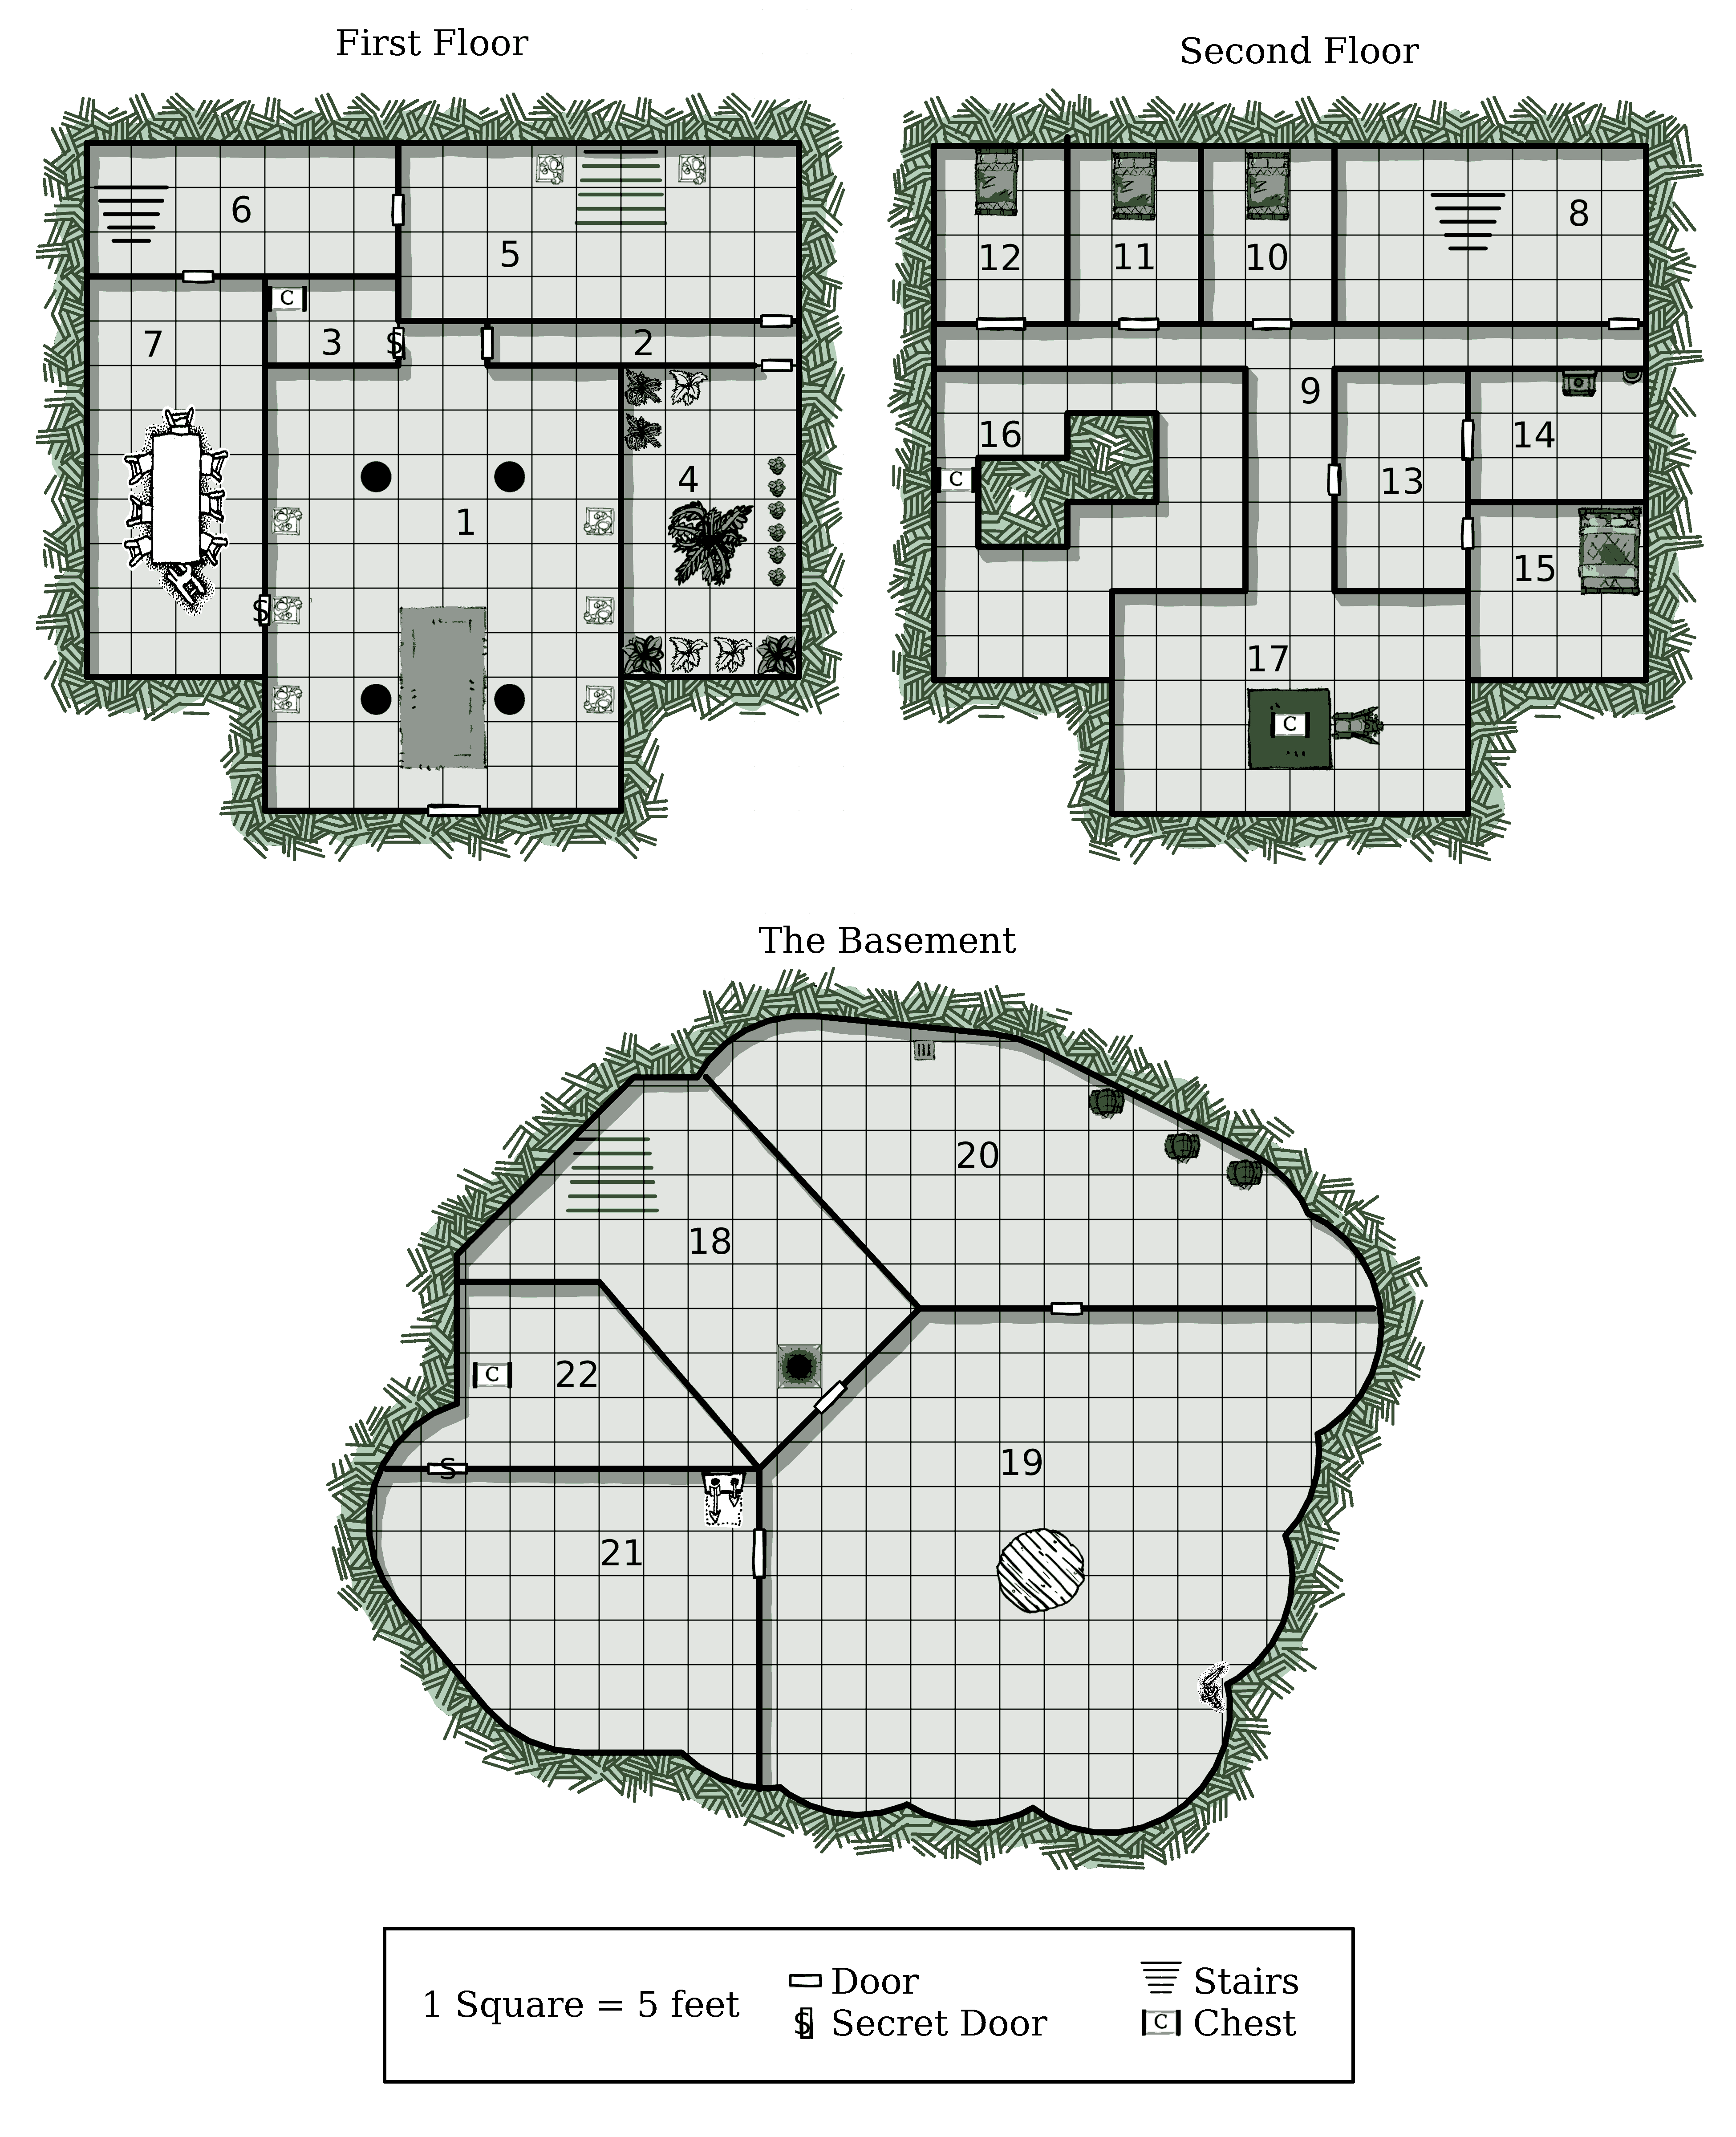
\includegraphics[width=\textwidth,height=0.9\textheight]{img/maps/ShakarrsMansion_45x45.png}
  \caption{Map 3.1 Shakarr's Vanishing Mansion}
\end{figure*}
\subsection{Conclusion}
The player's have explored the Vanishing Mansion of Shakarr. They are disappointed to not meet with the rumored wizard, and will have to continue in their voyages to search for intel about Amberia's brand. \\
Hopefully the players explored and were able to get some information about the world. By reading the notes in the Study, they should have received a clue that the owner of the mansion is connected to the Council of Seven. They could have learned about one of Malmalor Lumena's Curses, where she sabotaged one of Shakarr's experiments with time. They could have also gotten some foreshadowing about how Shakarr's memories are addled and out of order in time, which is why he recognizes them and runs away from them to begin with. And if they were very fortunate, they may have heard whispers of the underdark dwelling minions of the aberroth.\\
In the end, this dungeon should have provided the party with enough XP to reach Level 3, which should allow them to comfortably proceed on to the next adventure.
\section{The Aftermath}
The people of Garon City will be confused, but also relieved to see that the mansion that appeared one day has now disappeared just as suddenly, seemingly without causing them harm. Any townsfolk that recognize the party as adventurers might ask them about it. \\
If the party continue to ask around town for intel, the townsfolk should make it clear that they have no further information and encourage the party to seek the experts in Gold City.

%\chapter{The Cities of Silver and Gold}
%\chapter{The Blights}
%\chapter{Kiraki at War}
%\chapter{The Amcysian Invasion}
%\chapter{The Curse of Malmalor Lumena}
%\chapter{Gaelin's Schemes}

No schemes he's such a nice guy

%Resources
%\part{Resources}
\chapter{Brands}\label{Brands}
One of the major plot-hooks of the campaign centers around the divine brands. There are two ways a character can acquire a brand; they can take the Branded One background, or they can complete a special trial set by the god associated with the brand. Every person of one of the lineages created by the gods is eligible to have a patron god and take the Branded One background. Usually, a character's patron god is the same god as the one that created their lineage. There are exceptions to this, and it often makes for good roleplaying to explore why a god might have chosen one of your adventurers. The brands earned in trials can be acquired by any lineage, including those who are planar travelers and not one of the 16 lineages created by the gods of the plane.
\section{Branded One Background}\label{Branded One}
If your campaign intends to follow the main plothooks laid out in this guide, and your players are of a lineage created by the gods, they should take the Branded One background. This background grants them access to a brand which grants elemental magic associated with their patron god. As the Dungeon Master, you can choose to assign your player a patron god that fits with their backstory, or roll a d100 for each player taking the Branded One background and determine their god from the table below.
\begin{DndTable}[header=Brands,width=0.5\textwidth]{XX} 
Dice Roll & God \\
1-49 & The creator god of the character's lineage \\
50-59 & Shin \\
60-62 & Amalthea \\
63-65 & Daled \\
66-68 & Harpalyke \\
69-71 & Iona \\
72-74 & Khof \\
75-77 & Merope \\
78-80 & Praxidike \\
81-83 & Pasiphae \\
84-86 & Sinope \\
87-89 & Taygeta \\
90-92 & Themisto \\
93-95 & Tsadek \\
96 & Lysithea \\
97 & Meneas \\
98 & Taranis \\
99 & Tes \\
100 & Yarfinn \\
\end{DndTable}
Some gods are more common than others. Five gods in particular are much rarer than the others. Lysithea is very particular about only caring for orcs, her creation. Being selected by Lysithea as a non-orc character might mean she believes the character will be a great ally to the orcs.\\
Meneas's lineage, the Lurkers, are nearly extinct, and he spends his time trying to thwart the Restorationist Gods (see Chapter~). Being selected by Meneas might be he has a special mission or message to warn the character of the Restorationist Gods.\\
Taranis never created a race successfully, and cares little for mortals. Being selected by Taranis might mean he plans to use the character to bring about the restoration of the aberroth.\\
Tes has chosen to make her duty the re-purposing of the Immylium (or souls) of corpses and bringing them to new bodies. A character chosen by Tes might be selected with a purpose to destroy a person or force that is preventing Immylium from returning to the natural cycle of reincarnation.\\
Yarfinn, along with Taranis is the other restorationist god. He might choose a character if they believe the character can contribute to a world he believes rightfully belongs to the aberroth.\\
On the other hand, Shin is much more likely than other gods to patronize the other lineages. Shin created humans, but tries to avoid playing favorites.\\
\subsection{Branded One Features}
A character with the Branded One background has been marked by a Great Brander, a powerful shaman who can determine a person's patron god. When a character receives this mark, it appears in the form of a brand on their wrist, and grants them access to spells as their character levels up. At 1st level, the brand grants access to a cantrip, as shown in the table at the end of the chapter. At higher levels, the brand grants access to spells at the levels shown in the table. Each of these spells can be cast once, with no material components or focus needed, as long as the hand with the branded wrist is empty. You use your constitution as your spellcasting modifier for spells cast in this way. You regain the use of these spells after completing a long rest.
\newgeometry{left=0.2in,right=0.2in}
\begin{DndTable}[header=Brands,width=\textwidth]{XXXXXXXXXXXX} 

        \textbf{God} & \textbf{Lineage} & \textbf{Element} & \textbf{Level 1} & \textbf{Level 5} & \textbf{Level 9} & \textbf{Level 13} & \textbf{Level 17} &\textbf{Level 20}\\ \hline
        Amalthea & Elves & Illusion & Minor Illusion & Silent Image & Mirror Image & Fear & Hallucinatory Terrain & Mislead \\ 
        Daled & Crystallin & Ice & Frostbite & Frost Fingers & Snillloc’s Snowball Storm & Sleet Storm & Ice Storm & Cone of Cold \\ 
        Harpalyke & Aarakocra & Air & Gust & Feather Fall & Warding Wind & Fly & Summon (Air) Elemental & Freedom Of The Winds \\ 
        Iona & Flameblooded & Fire & Create Bonfire & Burning Hands & Aganazzer’s Scorcher & Ashardalon’s Stride & Fire Shield & Immolation \\
        Khof & Goblins & Alchemy and Infusion & Prestidigitation & Absorb Elements & Jim’s Glowing Coin & Remove Curse & Fabricate & Hallow \\ 
        Lysithea & Tieflings & Emotion & Friends & Cause Fear & Enthrall & Antagonize & Charm Monster & Dream \\ 
        Meneas & Lurkers & Shadows & Control Shadows* & Fog Cloud & Darkness & Hunger of Hadar & Shadow of Moil & Danse Macabre \\ 
        Merope & Arboreans & Plants & Thorn Whip & Entangle & Wither and Bloom & Plant Growth & Grasping Vine & Wrath of Nature \\ 
        Praxidike & Kobolds & Lightning & Lightning Lure & Thunderwave & Shatter & Lightning Bolt & Storm Sphere & Bolt Jump* \\ 
        Pasiphae & Dragonborn & Sound and Language & Thunderclap & Dissonant Whispers & Magic Mouth & Thunderstep & Choir of Angels* & Geas \\ 
        Shin & Humans & Health & Spare the Dying & Healing Word & Lesser Restoration & Mass Healing Word & Aura of Purity & Greater Restoration \\ 
        Sinope & Orcs & Combat & Primal Savagery & Zephyr Strike & Enlarge/ Reduce & Haste & Freedom Of Movement & Circle of Power \\ 
        Taranis & None & Light & Light & Chromatic Orb & Moonbeam & Daylight & Color Wheel* & Wall of Light \\ 
        Taygeta & Seafolk & Water & Shape Water & Create or Destroy Water & Lesser Water Walk* & Wall of Water & Watery Sphere & Maelstrom \\ 
        Tes & None & Death and Rebirth & Chill Touch & False Life & Gentle Repose & Summon Undead & Spirit of Death & Raise Dead \\ 
        Themisto & Gnomes & Metal & Sword Burst & Tenser’s Floating Disk & Heat Metal & Galder’s Tower & Leomond’s Secret Chest & Steel Wind Strike \\ 
        Tsadek & Fairies & Creatures & Infestation & Animal Friendship & Flock of Familiars & Conjure Animals & Find Greater Steed & Insect Plague \\ 
        Yarfinn & Dwarves & Stone and Earth & Mold Earth & Earth Tremor & Earthbind & Meld Into Stone & Stoneskin & Transmute Rock \\ 

\end{DndTable}
\small{* Spell mechanics listed in Chapter~\ref{Spells}}
\restoregeometry
%\include{Locations and One-shots}
%
\chapter{Monsters}\label{Monsters}
\DndDropCapLine{T}{he army of Amcys is equipped} with weapons more advanced than anywhere else on the continent.\\
% Monster stat block
\begin{DndMonster}[width=0.5\textwidth + 8pt]{Amcysian Rifleman}
    \DndMonsterType{Medium Human, Lawful Evil}

    % If you want to use commas in the key values, enclose the values in braces.
    \DndMonsterBasics[
        armor-class = {16},
        hit-points  = {\DndDice{7d10 + 2}},
        speed       = {30 ft.},
      ]

    \DndMonsterAbilityScores[
        str = 12,
        dex = 18,
        con = 14,
        int = 10,
        wis = 12,
        cha = 12,
      ]

    \DndMonsterDetails[
        saving-throws = {Dex +8, Wis +6},
        %skills = {Acrobatics +0, Animal Handling +0, Arcana +0, Athletics +0, Deception +0, History +0, Insight +0, Intimidation +0, Investigation +0, Medicine +0, Nature +0, Perception +0, Performance +0, Persuasion +0, Religion +0, Sleight of Hand +0, Stealth +0, Survival +0},
        %damage-vulnerabilities = {cold},
        %damage-resistances = {bludgeoning, piercing, and slashing from nonmagical attacks},
        %damage-immunities = {poison},
        %condition-immunities = {poisoned},
        senses = {passive Perception 15},
        languages = {Common},
        challenge = 2,
      ]
    % Traits
    

    \DndMonsterSection{Actions}
    \DndMonsterAction{Multiattack}
    The rifleman makes two ranged attacks.

    %Default values are shown commented out
    \DndMonsterAttack[
      name=Rifle,
      distance=ranged, % valid options are in the set {both,melee,ranged},
      %type=weapon, %valid options are in the set {weapon,spell}
      mod=+8,
      %reach=5,
      range=150/300,
      targets=one target,
      dmg=\DndDice{2d8+4},
      dmg-type=piercing,
      %plus-dmg=,
      %plus-dmg-type=,
      %or-dmg=,
      %or-dmg-when=,
      %extra=,
    ]

\end{DndMonster}

\begin{DndMonster}[float*=b,width=0.5\textwidth + 8pt]{Amcysian Lieutenant}
    \DndMonsterType{Medium Human, Lawful Evil}

    % If you want to use commas in the key values, enclose the values in braces.
    \DndMonsterBasics[
        armor-class = {18},
        hit-points  = {\DndDice{12d10 + 3}},
        speed       = {30 ft.},
      ]

    \DndMonsterAbilityScores[
        str = 12,
        dex = 20,
        con = 16,
        int = 10,
        wis = 12,
        cha = 12,
      ]

    \DndMonsterDetails[
        saving-throws = {Dex +10, Wis +8},
        skills = {Perception +5},
        %damage-vulnerabilities = {cold},
        damage-resistances = {bludgeoning, piercing, and slashing from nonmagical attacks},
        %damage-immunities = {poison},
        %condition-immunities = {poisoned},
        senses = {passive Perception 15},
        languages = {Common},
        challenge = 4,
      ]
    % Traits
    

    \DndMonsterSection{Actions}
    \DndMonsterAction{Multiattack}
    The lieutenant makes two ranged attacks with their rifle, or one with their sniper.

    %Default values are shown commented out
    \DndMonsterAttack[
      name=Rifle,
      distance=ranged, % valid options are in the set {both,melee,ranged},
      %type=weapon, %valid options are in the set {weapon,spell}
      mod=+10,
      %reach=5,
      range=150/300,
      targets=one target,
      dmg=\DndDice{2d8+5},
      dmg-type=piercing,
      %plus-dmg=,
      %plus-dmg-type=,
      %or-dmg=,
      %or-dmg-when=,
      %extra=,
    ]
    \DndMonsterAttack[
      name=Sniper,
      distance=ranged, % valid options are in the set {both,melee,ranged},
      %type=weapon, %valid options are in the set {weapon,spell}
      mod=+10,
      %reach=5,
      range=300/600,
      targets=one target,
      dmg=\DndDice{6d8+5},
      dmg-type=piercing,
      %plus-dmg=,
      %plus-dmg-type=,
      %or-dmg=,
      %or-dmg-when=,
      extra={, and this weapon will strike a critical hit with a dice roll of 19 as well as 20. This weapon has disadvantage if the target is within 100 ft}
    ]

\end{DndMonster}

\begin{DndMonster}[float*=b,width=0.5\textwidth + 8pt]{Angry Bed Sheet}
    \DndMonsterType{Medium Construct, Unaligned}

    % If you want to use commas in the key values, enclose the values in braces.
    \DndMonsterBasics[
        armor-class = {11},
        hit-points  = {\DndDice{3d8}},
        speed       = {10 ft.},
      ]

    \DndMonsterAbilityScores[
        str = 14,
        dex = 14,
        con = 10,
        int = 1,
        wis = 3,
        cha = 1,
      ]

    \DndMonsterDetails[
        %saving-throws = {Dex +10, Wis +8},
        %skills = {Acrobatics +0, Animal Handling +0, Arcana +0, Athletics +0, Deception +0, History +0, Insight +0, Intimidation +0, Investigation +0, Medicine +0, Nature +0, Perception +0, Performance +0, Persuasion +0, Religion +0, Sleight of Hand +0, Stealth +0, Survival +0},
        %damage-vulnerabilities = {cold},
        damage-resistances = {bludgeoning, piercing, and slashing from nonmagical attacks},
        %damage-immunities = {poison},
        condition-immunities = {Blinded, Charmed, Deafened, Frightened, Paralyzed, Petrified, Poisoned},
        senses = {Blindsight 60 ft. (blind beyond this radius), Passive Perception 6},
        languages = {--},
        challenge = 1/4,
      ]
    % Traits
    \DndMonsterAction{Antimagic Susceptibility} The bed sheet is incapacitated while in the area of an antimagic field. If targeted by dispel magic, the bed sheet must succeed on a Constitution saving throw against the caster's spell save DC or fall unconscious for 1 minute.
    \DndMonsterAction{Damage Transfer} While it is grappling a creature, the bed sheet takes only half the damage dealt to it, and the creature grappled by the bed sheet takes the other half.
    \DndMonsterAction{False Appearance} While the rug remains motionless, it is indistinguishable from a normal rug.

    \DndMonsterSection{Actions}
    %Default values are shown commented out
    \DndMonsterAttack[
      name=Smother,
      distance=melee, % valid options are in the set {both,melee,ranged},
      %type=weapon, %valid options are in the set {weapon,spell}
      mod=+4,
      reach=5,
      %range=150/300,
      targets=one medium or smaller creature,
      %dmg=\DndDice{1d6+2},
      %dmg-type=bludgeoning,
      %plus-dmg=,
      %plus-dmg-type=,
      %or-dmg=,
      %or-dmg-when=,
      extra={The creature is grappled (escape DC 13). Until this grapple ends, the target is restrained, blinded, and at risk of suffocating, and the bed sheet can't smother another target. In addition, at the start of each of the target's turns, the target takes 1d6+2 bludgeoning damage.}
    ]
   
\end{DndMonster}
\begin{DndMonster}[float*=b,width=0.5\textwidth + 8pt]{Color Eater}
    \DndMonsterType{Medium Monstrosity, Neutral Evil}

    % If you want to use commas in the key values, enclose the values in braces.
    \DndMonsterBasics[
        armor-class = {14},
        hit-points  = {\DndDice{7d10+14}},
        speed       = {30 ft.},
      ]

    \DndMonsterAbilityScores[
        str = 7,
        dex = 14,
        con = 14,
        int = 16,
        wis = 14,
        cha = 20,
      ]

    \DndMonsterDetails[
        saving-throws = {Dex +5, Wis +5},
        skills = {Performance +8, Stealth +5},
        %damage-vulnerabilities = {cold},
        %damage-resistances = {bludgeoning, piercing, and slashing from nonmagical attacks},
        %damage-immunities = {poison},
        condition-immunities = {Blinded},
        senses = {passive Perception 12},
        languages = {Common},
        challenge = 6,
      ]
    % Traits
    
    \DndMonsterAction{Color Shield} The Color Eater cannot be damaged by any attacks or spells that are of a mostly colorless pigmentation such as black, white, silver, or grey (this includes most bladed weapons or natural claws.)
    \DndMonsterAction{Spellcasting} The Color Eater is a 7th level spellcaster. Its spellcasting ability is Charisma (spell DC 16, +8 to hit with spell attacks), and it can cast Color Wheel at will as a 4th level spell.\\
    \noindent 1st Level (3 Slots): \textit{Absorb Elements}\\
    \noindent 2nd Level (2 Slots): \textit{Color Spray}\\ 
    \noindent 3rd Level (2 Slots): \textit{Hypnotic Pattern}\\
    \noindent 4th Level (1 Slot): \textit{Vitriolic Sphere, Color Wheel} (which can be cast at will)\\
    
    \DndMonsterSection{Actions}
    %Default values are shown commented out
    \DndMonsterAttack[
      name=Color Siphon,
      distance=ranged, % valid options are in the set {both,melee,ranged},
      %type=weapon, %valid options are in the set {weapon,spell}
      mod=+8,
      %reach=5,
      range=15,
      targets=one creature,
      dmg=\DndDice{4d8+5},
      dmg-type=psychic,
      %plus-dmg=,
      %plus-dmg-type=,
      %or-dmg=,
      %or-dmg-when=,
      extra={The target is siphoned of it ability to wield any objects or produce any effects or spells that create the color which matches the current shade of the Color Eater for 24 hours. Non-magical, non-living objects on the target such as clothes which are of the color siphoned permanently lose their color. All colors fall into the category of either red, orange, yellow, green, blue, purple, black, white, or grey at the DM's discretion. The color eater regains a number of hit points equal to the number of distinct items of this color are on the target, up to a maximum of 10}
    ]
    \\
    
   \DndMonsterSection{Bonus Actions}
   \DndMonsterAction{Color Change} The Color Eater can change its color. The color choices are red, orange, yellow, green, blue, or purple.
   \DndMonsterAction{Shapechange} The Color Eater can assume the form of any humanoid it has seen, or revert to its true form. It cannot use any of its other abilities in a humanoid form.
\end{DndMonster}
%\chapter{Random Encounters}
\begin{DndTable}[header=Western Kiraki, width=0.45\textwidth]{M|XXX}
    \textbf{Party Level}  & \textbf{Dice Roll} & \textbf{Enemies} & \textbf{XP} & \textbf{Treasure} \\
    1 & 1 & 2 Blink Dogs & 100 &\\
    & 2 & 3 Orcs \\

\end{DndTable}  
\hfill \break
\chapter{New Playable Races}\label{Races}
\section{Arborean}
\DndDropCapLine{A}{wondrous species, isolated but loyal.} \textit{Though their race lives in the woods not but a few miles from my home, I rarely get chance to see one up close. Outside of us tieflings, arboreans seem to be the most saddened by the treatment of the orcs. I hope to forge an alliance with them. I shall seek them out east of Belondir.}\\
 \begin{flushright}---Malmalor Lumena \end{flushright}
The woods are a place where every sentient being knows: \textit{I am not alone}. There are animals of all scales, some predators, and some prey. A traveler's eyes and ears will scan for dangers, for in the forest there are many. Dark magics can collect in forgotten forests, and so arboreans make sure the forests are not forgotten.\\
Arboreans are tree-like beings, with rough bark for skin.
\subsection{Merope's Chosen}
Merope, inspired by the bountiful green life of the material plane drew heavy inspiration from trees when she developed her Chosen Race. The goddess of plants and nature drew heavy inspiration from trees when crafting Oaknaught, the first arborean. Seeing the efficient design of the bipedal forms her fellow gods had created, Merope followed suit, but made sure to preserve that which inspired her about trees: their hardy bark, their greenery, and most of all their peaceful nature.\\
Like the trees they were inspired from, Merope chose to make Arboreans varied, adapted to the specific environment of their creation. In the hardy deciduous forests of southern Kiraki, hardwood arboreans patrol the Belondir Glades, keeping them clear of underbrush with plenty of space for sunlight to break through. In the orchards and farmlands of central Kiraki, fruiting arboreans are plentiful and cheery. In the frigid snowy mountains where only conifers thrive, evergreen arboreans ensure that their forests do not fall prey to avalanches. In the lush jungles north of Obron Village, and in Tadau Kotoru, Palmetto arboreans sway in the breeze and enjoy the sun. Petrified wood arboreans aimlessly roam near the bogs around Barium Cemetery, a spark of (un)life that Merope did not intend.
\subsection{Shepherds of the Forest}

\subsection{Arborean Traits}
Your Arborean Character has a variety of natural properties and abilities, owing to its treelike properties and close connection to nature.
\subparagraph{Ability Score Increase}Your Constitution score increases by 2.
\subparagraph{Age}Arboreans reach physical maturity around 25, then typically live up to 300 years old.
\subparagraph{Alignment}Arboreans tend to neutral good alignments, though if their forests have been damaged they can venture into chaotic evil territory as they seek vengeance upon those who hurt their forests.
\subparagraph{Size}Arboreans tend to be between 7 and 8 feet tall, and weigh between 400 and 800 pounds. Your size is Medium.
\subparagraph{Creature Type}You count as both a humanoid and plant creature.
\subparagraph{Speed}Your base walking speed is 25 feet. 
\subparagraph{Photosynthesis}As long as you receive four hours of sunlight in a day, you do not need to eat. Going without sunlight for longer than a week will give a level of exhaustion. An additional point of exhaustion is gained for each week spent without sunlight.
\subparagraph{Rootsense}You can sense the location of any creature making contact with nonmagical unworked earth within 30 feet.
\subparagraph{Bark}Your AC increases by 1, and you have resistance to non-magical bludgeoning damage. You have susceptibility to fire damage, and spells or attacks involving fire damage ignore this bonus to AC. You can still gain the normal benefits of a shield if otherwise allowed.
\subparagraph{Languages}You can speak and read Common, Druidic, and Arborean. Arborean is a low guttural language that takes many minutes to communicate what other languages could communicate in a short sentence.
\subparagraph{Subrace}
There are several subraces of arboreans. Choose one.
\begin{DndSidebar}[float=!b]{Peoples of the Woods}
  Arboreans are one of the seven races represented by Kiraki's Council of Seven. They are the pet creation of Merope, goddess of plants, and they act accordingly. Arboreans dedicate their lives to preserving forests. Of all of the races created by the gods of Sunday, arboreans are probably the most welcomed anywhere they are found.
\end{DndSidebar}
\subsubsection{Hardwood Arborean}
Hardwood Arboreans live in the southern forests of Kiraki, as well as in other hardy deciduous forests throughout the continent of Sunday. They are in tune with the seasonal changes of the world, and can present in four different forms depending on which seasonal affect feels appropriate to them. Hardwood arboreans have extremely protective instincts over their home forest, and will go to extreme lengths to protect the ecosystems there.
\subparagraph{Ability Score Increase}Your Strength score increases by 1.
\subparagraph{Extra Sturdy}When you are not wearing armour, your base AC increases by an additional 1, for a total of +2, with all of the other rules of Bark applied to this bonus.
\subparagraph{Seasonal Form}Over the course of a long rest, you can choose whether or not to advance your seasonal appearance to a different one of the four seasonal forms you can take, which each grant a different ability. Your season does not need to match the real world season, but a hardwood arborean usually chooses to present this way unless great need dictates otherwise.
\subparagraph{Spring Form}\textit{New Life:} You can use a bonus action to regain a number of hit points equal to your level. You can do this three times per long rest.
\subparagraph{Summer Form}\textit{Animal Companion:} An animal companion will take roost in your branches. You can cast Find Familiar as an action once per long rest without using a spell slot. The familiar disappears after a number of hours equal to half your level, rounded up.
\subparagraph{Autumn Form}\textit{Vibrant Foliage:} Your entrancing appearance causes you to gain proficiency in Persuasion, Deception, and Performance checks while you are in this seasonal form.
\subparagraph{Winter Form}\textit{Unburdened:} Without leaves to slow you down, your speed increases by 10 ft.

\subsubsection{Evergreen Arborean}
Evergreen arboreans tend to live in the coniferous forests along the mountain ranges bordering Kiraki. Their needly exterior keeps others at bay, which is just the way they like it. They are the most insular type of Arborean, and are rarely found wandering into cities. They can be mistrusting, but are usually fiercly loyal once friendship is established.
\subparagraph{Ability Score Increase}Your Wisdom score increases by 1.
\subparagraph{Spiky}Your needled exterior causes all enemy creatures who make contact with you, or make successful melee attacks against you from within 5 feet of you to make a Dexterity saving through (DC 10+proficiency). On a fail, they take 1d6 piercing damage. A creature can only take damage from this effect once per round.
\subparagraph{Pitch}As an action, you spray the ground within a 30 ft radius circle of you with sticky pitch, making it difficult terrain for non-plant creatures. You can use this feature twice per long rest.

\subsubsection{Palmetto Arborean}
Guardians of the jungles and palm forests near Obron Village in Kiraki, as well as on the Island of Piva Pava, and the nation of Tadau Koturu, Palmetto arboreans are the most outgoing of the arborean subraces. They will leave their forests to party and celebrate, and are known for their elegant dancing.
\subparagraph{Ability Score Increase}Your Dexterity score increases by 1.
\subparagraph{Stormweathered}You are unshakeable, and can choose to be unaffected by any spells or effects involving being moved or damaged by wind. You also have resistance to force damage.
\subparagraph{Coconut Drop}As a reaction to being hit with a melee attack, you can choose to drop a coconut from height on the attacker. The attacker takes 1d8 bludgeoning damage. Additionally, if the creature has a head and is not wearing a helmet, and the creature is of the same size or smaller than you (or its head is below yours), it must make a Constitution saving throw (DC = 8 + your Constitution modifier + your proficiency bonus) or be stunned for one round. You can use this feature twice, and it recharges after a long rest.

\subsubsection{Fruiting Arborean}
Native to the wooded areas near the farmlands in north and central Kiraki, as well as in Sunnudagar and Nedelja, fruiting arboreans are known for their generosity and kind nature. They often shepherd small troops of animals and keep them fed from their fruit. When they wander into civilization, they are greeted with celebration and joy.
\subparagraph{Ability Score Increase}Your Charisma score increases by 1.
\subparagraph{Fruiting Bounty}As long as you have a long-rest over fertile soil, and have taken in at least four hours of sunlight within the last week, you can produce enough fruit to feed one person from each of your four limbs. The type of fruit is set from birth, unless you graft a limb from another fruiting arborean. The fruit eaten will grant the consumer an additional bonus. It takes one minute to eat the fruits, and the advantage the fruit grants lasts two hours.\\
\textit{Peach: }Those who eat your fruits gain advantage on Charisma Saving throws.\\
\textit{Apple: }Those who eat your fruits gain advantage on Intelligence Saving throws.\\
\textit{Pecan: }Those who eat your fruits gain advantage on Constitution Saving throws.\\
\textit{Cherry: }Those who eat your fruits gain advantage on Dexterity Saving throws.\\
\textit{Pear: }Those who eat your fruits gain advantage on Wisdom Saving throws.\\
\textit{Grapefruit: }Those who eat your fruits get advantage on Strength Saving throws.\\
\subparagraph{Grafting}You can gain the fruiting bounties of other Fruiting Arboreans. You can do this by choosing to exchange a limb with them. The fruit off of each limb can feed one person enough to gain the benefit. The limb will take 2d4 days to heal and function properly again. If it is an arm, you will be unable to hold weapons or other items heavier than one pound until it is healed. If it is a leg, your speed is halved and you automatically fail Dexterity based saving throws until it is healed.
\subsubsection{Petrified Wood Arborean}
Deep beneath the muddy bogs to the north of Barium Cemetery, dead trees became petrified, and then were resurrected as undead arboreans. These arboreans aimlessly roam Barium Cemetery looking for purpose, not accepted by most of their kind.
\subparagraph{Ability Score Increase}Your Intelligence Score Increases by 1.
\subparagraph{Languages}You are fluent in Undercommon rather than Druidic.
\subparagraph{Creature Type}Rather than count as a plant creature, you count as undead, as well as humanoid.
\subparagraph{Fossilized}You resist, rather than have susceptibility to fire damage.
\subparagraph{Darkvision}Resurrected in the caves below sunken bogs, rather than \textbf{Rootsense}, you have superior vision in dark and dim conditions. You can see in dim light within 60 feet of you as if it were bright light, and in darkness as if it were dim light. You can’t discern color in darkness, only shades of gray.
\raggedbottom
\pagebreak
\section{Crystallin}
Crystallin are a rare and enigmatic race of humanoid beings with ice-blue skin, giving them an ethereal and otherworldly appearance. Their most distinctive feature is the shards of a shimmering, ice-like material that protrude from their spines, glistening like diamonds in the sunlight. Crystallin are a hardy people, well-suited to the harsh and frigid mountain environments where they make their homes.
\subsection{Carnivorous Hunters}
Crystallin are strict carnivores, feeding exclusively on the meat of mountain creatures that they hunt and trap. They have evolved to survive in areas where plant life is scarce, and their bodies are able to derive all the nutrients they need from the flesh of their prey. This has led them to develop a unique culture around the hunting and preparation of meat, with elaborate rituals and ceremonies surrounding the consumption of each kill.\\
Crystallin are a solitary people, preferring to live in small, tight-knit communities scattered across the mountains. They believe in self-sufficiency, with each individual responsible for their own survival. This has led to a culture of individualism, with each Crystallin honing their skills as hunters, trappers, and craftsmen.\\
Crystallin are skilled in the use of weapons made from the ice-like material that protrudes from their spines. They fashion sharp, deadly blades and spears, as well as powerful shields that can withstand even the strongest blows. They also have a deep understanding of ice, which they use to shape the frozen landscape around them.\\
Crystallin are wary of outsiders, preferring to keep to themselves and protect their way of life. However, those who are able to earn their trust are welcomed with open arms, and the Crystallin are fiercely loyal to their allies. They are a people of great strength and resilience, shaped by the harsh and unforgiving environment in which they live.
\subsection{Crystallin Traits}
Your Crystallin Character has a variety of abilities originating from its connection to Daled, the god of ice.
\subparagraph{Ability Score Increase}Your Constitution score increases by 2 and your Intelligence score increases by 1.
\subparagraph{Age}Crystallin reach physical maturity around 16, then typically live up to 80 years old.
\subparagraph{Alignment}Crystallin often tend towards neutral alignments. They tend to value their clan first, but are rarely outright cruel.
\subparagraph{Size}Crystallin tend to be between 5 and a half and 6 and a half feet tall, and weigh between 180 and 260 pounds. Your size is Medium.
\subparagraph{Speed}Your base walking speed is 30 feet.
\subparagraph{Hunter's Nature} You have advantage on Survival checks and Investigation or Perception checks that involve tracking creatures.
\subparagraph{Blood of Ice} You have resistance to cold damage. Any creature that grapples you or restrains you with its body must make a Constitution saving throw (DC = 8 + your Consitution modifier + your proficiency bonus) or take 1d8 cold damage for every turn it is in contact with you. 
\subparagraph{Spine Shards} The icy shards which grow from your spine erupt off of your body. When you take the Attack action, you can replace one of your attacks with your Spine Shards. All creatures in a 15 foot cone must make a Dexterity saving throw (DC = 8 + your Consitution modifier + your proficiency bonus), taking 1d10 cold damage on a failed save, or half as much on a successful save. This damage increases by 1d10 when you reach 5th level (2d10), 11th level (3d10), and 17th level (4d10) You can use this feature a number of times equal to your proficiency bonus, and regain use of it after a long rest.
\subparagraph{Languages}You can speak, read, and write Common and Crystallin.

\raggedbottom
\pagebreak

\section{Flameblooded}
\textit{As I stood at the edge of the clearing, I watched with a mix of awe and trepidation as a figure emerged from a cloud of smoke. The woman's skin glowed a fiery orange, and her eyes eyes were fixed upon me with a predatory intensity, as she twirled two gleaming daggers in he hands. The flameblooded moved with a grace and fluidity that I had never seen before, as if the daggers were simply an extension of their own body.\\
I knew my belongings would not be mine for much longer, but still I could not help be captivated by the glow of the woman, as she approached, as fluid as smoke. Her confidence, her assertiveness, made me believe that I could have some of mine own.} \\ \begin{flushright}---Malmalor Lumena \end{flushright}
\subsection{Iona's Children}
 Iona, the goddess of fire and destruction, was believed to have infused her own divine essence into the very veins of her Chosen Race. Legend has it that Iona created the flameblooded to be her loyal followers and warriors, imbuing them with the power of fire and passion to serve as her champions.\\
Flameblooded are characterized by their distinct physical features, including yellow to orange skin, bright fiery eyes, and hair that shimmers like flames in the sunlight. Their veins run with a primordial fire, giving them a natural affinity for flames, and the ability to control and manipulate them to their will. They are also known for their incredible endurance and resilience to heat, which allow them to thrive in the harsh desert environment they call home.\\
The flameblooded have a rich cultural history, centered around their devotion to Iona and their belief in the power of fire to cleanse and purify. They are deeply connected to the land they inhabit, and view the desert as a place of spiritual renewal and transformation. They are fierce warriors and skilled craftspeople, known for their intricate metalworking and jewelry-making skills, which often feature fiery motifs and designs inspired by their connection to the flame. Despite their intense devotion to Iona and the power of fire, flameblooded are also known for their passionate and tempestuous natures.
\subsection{A Charred Soul}
Coal holds a special significance in the rituals of the flameblooded. As a race that is inherently connected to the power of fire, coal is seen as a symbol of transformation and purification. During important ceremonies and rituals, flameblooded will often use coal to create large fires of purification. The heat and light of the flames are believed to awaken the innate power of the flameblooded, allowing them to connect more deeply with Iona.\\
In addition to its symbolic importance, coal is also used practically in many aspects of flameblooded life. The harsh desert environment in which they live often makes it difficult to find reliable sources of fuel for cooking and heating, and coal provides a steady and long-lasting source of heat. It is also used in the creation of their intricate metalworking, which often features fiery motifs and designs. For the flameblooded, coal is both a practical necessity and a powerful symbol of their connection to the divine power of fire.
\subsection{Life on the Road}
The flameblooded, despite settling in cities, have a tendency to lead a life of wandering. Their wanderlust nature often leads them to reject the confines of settled society in favor of a more nomadic existence. However, their penchant for independence often leads them astray, and many of them are known to succumb to a life of piracy and other forms of roguish activity.\\
Their natural connection to fire and formidable strength makes the flameblooded a formidable force in combat, which often makes them attractive candidates for a life of adventure and danger. Their sense of loyalty and duty to their own people often binds them together, making them an unstoppable force that few would dare cross. This reputation has earned them admiration and respect, and many consider them to be living embodiments of the free spirit of fire.\\
However, this wandering lifestyle often puts them at odds with settled societies, and they may be seen as outsiders and troublemakers. The flameblooded's tendency towards banditry often puts them at odds with law enforcement and other powerful groups that seek to bring them to justice. Despite these risks, many flameblooded continue to embrace the life of a wanderer, seeing it as the only true path to freedom and independence.
\subsection{Flameblooded Traits}
\subparagraph{Ability Score Increase}Your Charisma score increases by 2 and your Dexterity score increases by 1.
\subparagraph{Age}Flameblooded age in a similar manner to humans, reaching physical maturity around 18, and then usually live from 75 to 100 years.
\subparagraph{Alignment}Flameblooded have hot tempers, and tend to chaotic alignments.
\subparagraph{Size}Flameblooded are of a similar size to humans, ranging from 5 to 6 feet tall, and 130 to 180 pounds. Your size is Medium. 
\subparagraph{Speed}Your base walking speed is 30 feet. 
\subparagraph{Darkvision} You can see in dim light within 60 feet of you as if it were bright light, and in darkness as if it were dim light. You can't discern color in darkness, only shades of gray.
\subparagraph{Blood of Fire} You have resistance to fire damage. Any creature that grapples you or restrains you with its body must make a Constitution saving throw (DC = 8 + your Consitution modifier + your proficiency bonus) or take 1d8 fire damage for every turn it is in contact with you. 
\subparagraph{Scalding Sword} Your melee weapons which are made of metal deal an extra 1d4 fire damage. You cannot gain this benefit if the weapon has wooden parts or if the handle is not made of metal.
\subparagraph{Languages}You can speak, read, and write Common and Ignan.
\section{Lurkers}
\section{Seafolk}

\chapter{New Playable Class and Subclasses}\label{Mentalist}
\section{Mentalist}

An arborean bends down, inspecting the muddy ground. The subtle outline of imprints is all that he needs to pursue the poachers who set flame to his forest. A human woman reaches her arm out, just in time to stop the king from taking a sip. The faintest difference in hue is all it takes for this observant servant to spot the poison in the drink. An aged tiefling man lashes out with his cane, striking the orc in the weak spot between the joints of her armor that only he noticed. He predicts her retaliation, and despite his elderly body, effortlessly dodges a devastating blow.

\subsection{Detectives and Investigators}

Every great Rogue Thief will eventually draw the attention of an equally great detective, determined to track them down. Some do it for the sense of justice, but many do it purely for the thrill of solving a great mystery. Mentalists, known for their exceptional cleverness, perceive the world as inherently predictable. They employ their brilliant logical skills to effectively track and pursue their targets.

Lords and sheriffs frequently extend substantial rewards for the services of a Mentalist, yet a Mentalist selectively chooses cases that captivate their interest. Financial support is seldom a concern for a Mentalist. If they prioritized wealth, their talents could be employed to discern the subtle facial cues of unsuspecting gamblers and amass substantial fortunes.

\subsection{Seeing What Others Miss}

Mentalists inherently observe their surroundings with acute awareness. Occasionally, this heightened sensitivity becomes overwhelming as their senses absorb more than the average person's. Identifying traps and ambushes pose little challenge for a Mentalist. Even during sleep, a Mentalist's body remains vigilant, discerning the slightest changes in the sounds of nearby wildlife.

In combat, many Mentalists might seem physically outmatched, but they are rarely outwitted. They possess the ability to discern a monster's vulnerabilities, enabling a well-aimed strike with a mere walking stick or cane to inflict severe damage. A Mentalist can anticipate and counter a spellcaster's attacks or glean a target's deepest fears from their body language.

A Mentalist will never let the same enemy get the best of them twice. If an enemy escapes or bests them once, a Mentalist will replay the moment in their mind until they have determined how to prevent the same from happening again.

\subsection{Creating a Mentalist}

Mentalists are not crafted; instead, they are born with a preternatural gift, allowing them to perceive the world as it truly is. While inherently brilliant, Mentalists frequently grapple with a certain degree of antisocial tendencies. Their awareness of the flaws and secrets of those they encounter often taints their perspective of people and society with a negative hue.

Perhaps your character traverses the world in search of anything intriguing to alleviate the existential boredom of loneliness. Alternatively, they may be on a quest to find the one criminal who has successfully outwitted them. Is your Mentalist harboring anger toward the world, or are they fascinated by its intricacies? Do they revel in showcasing their talents, or do they prefer to keep their abilities private? Can your Mentalist foster close relationships with others when every secret flaw is laid bare to their heightened perception?

 \subsubsection{Quick Build}
 You can make a Mentalist quickly by following these suggestions. First, Intelligence should be your highest score, followed by Dexterity, then Charisma. Second, if you are not choosing the Branded background in the Kiraki Campaign setting, choose the Folk Hero or Sage background.
 \section{Class Features}
 As a Mentalist, you gain the following class features.
\subsubsection{Hit Points}
\noindent\textbf{Hit Dice:} 1d8 per Mentalist level\\
\noindent\textbf{Hit Points at 1st Level:} 8 + your Constitution modifier\\
\noindent\textbf{Hit Points at Higher Levels:} 1d8 (or 5) + your Constitution modifier per Mentalist level after 1st

\subsubsection{Proficiencies}
\noindent\textbf{Armor:} None\\
\noindent\textbf{Weapons:} Canes, walking sticks, or other similarly styled Mentalist Weapons\\
\noindent\textbf{Tools:} Thieves' Tools or Forgery Kit\\
\noindent\textbf{Saving Throws:} Intelligence, Charisma\\
\noindent\textbf{Skills:} Choose four from Perception, Investigation, History, Insight, Persuasion, Deception, and Intimidation

\subsubsection{Equipment}
You start with the following equipment, in addition to the equipment granted by your background:
\begin{itemize}
  \item A cane, walking stick, or pointer stick, which serves as your Mentalist Weapon for striking enemies in their most vulnerable locations.
  \item (a) any simple weapon, or (b) 2 daggers
  \item (a) an adventurer's pack, or (b) a burglar’s pack
\end{itemize}


\subsubsection{Stick Fighting}
At 1st level, your intuition and meticulous study of anatomy allow you to strike at creatures in their most vulnerable spots using a simple stick or cane. The cane is considered a light, simple Mentalist Weapon, dealing non-magical bludgeoning damage. You can only wield one Mentalist Weapon. The damage of the Mentalist Weapon is determined by the character's Mentalist level, as shown in the Mentalist table.

While wielding only your Mentalist Weapon (without a shield, other weapons, or focuses), you gain the following benefits:
\begin{itemize}
    \item You can add your Intelligence modifier as well as your Dexterity modifier to both your attack and damage rolls.
    \item For creatures with no levels in Mentalist, a Mentalist Weapon deals a flat 1d4 damage.
\end{itemize}
\subsubsection{Unarmored Defense}
At 1st level, when you are not wearing any armor and not wielding a shield, your Armor Class equals 10 + your Dexterity modifier + your Intelligence modifier.
\subsubsection{Keen Eye} 
At 2nd level, your accelerated information processing grants you advantage on Perception, Investigation, and Insight checks.
\subsubsection{Anticipation} 
At 2nd level, you acquire the ability to take the Dodge action as a bonus action a number of times equal to your proficiency bonus. You regain all uses of this feature after a short or long rest.
\subsubsection{Logical Mind} 
At 4th level, you become immune to the Charmed condition.

At 9th level, you become immune to being Frightened.
\begin{DndTable}[header=The Mentalist, width=0.59\textwidth]{m{0.04\textwidth}m{0.07\textwidth}m{0.06\textwidth}m{0.2\textwidth}}
    \textbf{Level}  & \textbf{Proficiency Bonus} & \textbf{Mentalist Weapon Damage} & \textbf{Features}\\
    1st  & +2 & 1d4 & Unarmored Defense, Stick Fighting\\
    2nd & +2 & 1d4 & Keen Eye, Anticipation\\
    3rd & +2 & 1d4 & Mentalist Specialty \\
    4th & +2 & 1d6 & Ability Score Improvement, Logical Mind\\
    5th & +3 & 1d6 & Extra Attack, Deduction \\
    6th & +3 & 1d6 & Mentalist Specialty Feature\\
    7th & +3 & 1d6 & Observist, Watchful Eyes\\
    8th & +3 & 1d6 & Ability Score Improvement \\
    9th & +4 & 2d4 & Logical Mind Improvement, Unavoidable presence \\
    10th & +4 & 2d4 & Precise Attack \\
    11th & +4 & 2d4 & Mentalist Specialty Feature \\
    12th & +4 & 2d4 & Extra Attack \\
    13th & +5 & 2d4 & Act Natural \\
    14th & +5 & 2d4 & Watchful Eyes Improvement \\
    15th & +5 & 2d4 & Let's Try That Again \\
    16th & +5 & 2d4 & Ability Score Improvement \\
    17th & +6 & 1d4+1d6 & Mentalist Specialty Feature \\
    18th & +6 & 1d4+1d6 & True Understanding \\
    19th & +6 & 1d4+1d6 & Ability Score Improvement \\
    20th & +6 & 1d4+1d6 & Predictive Master \\
\end{DndTable}  
\subsubsection{Extra Attack}
At 5th level, you gain the ability to make a second strike with your Mentalist Weapon as part of your attack action.

At 12th level, this capability increases, allowing you to make a third strike with your Mentalist Weapon as part of your attack action.
\subsubsection{Deduction}
At 5th level, you can utilize your bonus action to attempt to discern all of a creature's resistances, immunities, and susceptibilities. Make an insight check with a DC equal to the creature’s (CR/level + 10) to have this information revealed to you.
\subsubsection{Observist}
At 7th level, your mastery of observation and reflection grants you a significant advantage. If you have previously fought an individual or an identical enemy, you gain advantage on all attacks against that being, provided you have taken the time to reflect during a short or long rest in between encounters. Creatures are considered identical if they belong to the same species and have an Intelligence score lower than 10.
\subsubsection{Watchful Eyes}
At 7th level, your passive perception cannot be lower than 18. Additionally, you automatically detect any traps with a DC lower than 16.

At 14th level, your passive perception cannot be lower than 20, irrespective of your Wisdom modifier. When you roll to detect any traps, treat any dice roll at or below a 9 as a 10. In addition, you cannot be surprised.
\subsubsection{Unavoidable Presence}
At 9th level, the reach of your Mentalist Weapon extends to 10 feet. Additionally, you gain the flanking bonus if any ally is within 10 feet of the target, even if positioning would not typically grant flanking. Furthermore, your Mentalist Weapon attacks are now considered magical.
\subsubsection{Precise Attack}
At 10th level, when you score a critical hit, both the dice rolls and the flat damage modifiers are doubled.
\subsubsection{Act Natural}
At 13th level, you can use a bonus action to take the Hide action.

Outside of combat, you can seamlessly blend into the environment, making it appear as if you are a natural part of the surroundings to an enemy you have not directly engaged. A creature must have a passive Perception higher than 20 or actively be on the lookout, making a successful DC 17 Wisdom (Perception) check to become aware of your presence.
\subsubsection{Let's Try That Again}
At 15th level, you gain the ability to prefigure conversations before they occur. If an non-combat interaction with a creature turns unfavorable, you can designate the last minute of this conversation or interaction as a prediction and then resume the conversation or interaction from one minute earlier. You can use this feature once and regain its use after a short or long rest.
\subsubsection{True Understanding}
At 18th level, your understanding of what makes a creature tick is so profound that you can dismantle its identity with just a few words. You can take an action to compel a target within hearing range of you to make a Wisdom saving throw (DC 10 + your Charisma modifier + your Intelligence modifier). The creature takes 80 psychic damage on a failed save, or half as much on a successful one. To use this feature, you must have observed the creature for more than one minute, the target's Intelligence score must be greater than 6, and the target must be able to hear and understand you. You regain the use of this feature after a long rest.
\subsubsection{Predictive Master}
At 20th level, you can utilize your reaction at the start of a round of combat to foresee the precise unfolding of the entire round. You influence the flow, causing all enemies to miss all attacks directed against you or allies within 10 feet of you for the entire round. Additionally, you effortlessly pass all saving throws during the round. You regain the use of this feature after a short rest.
\section{Mentalist Observation Specialties}
At 3rd level, you learn to specialize in one type of observation and this gains you features at 3rd level and again at 6th, 11th, and 17th level. 
\subsection{Observer of Body}
You've dedicated yourself to the prediction and anticipation of attacks, investing years in studying the physiology of both humanoid and monstrous adversaries. Your expertise enhances your ability to evade and strike against non-magical creatures.
\subsubsection{Can't Touch This}
At 3rd level, you acquire the skill to roll with advantage against any effects stemming from a non-magical attack or contact by a creature that necessitates Strength or Dexterity-based saving throws or contested ability checks. Additionally, you gain proficiency in the Acrobatics and Athletics skills.
\subsubsection{Find the Weak Point}
At 6th level, you develop an understanding of creatures' pressure points, allowing you to inflict maximum damage. The dice roll you need to score a critical hit is reduced by 1, and you can bypass an enemy's resistance to your damage types.
\subsubsection{Unarmored Defense Improvement}
At 11th level your unarmored AC increases by 2.
\subsubsection{Stunning Smack}
At 17th level, upon the first successful hit of the round with your Mentalist Weapon, the targeted creature must succeed on a Constitution saving throw (DC 6 + your Intelligence modifier + your Dexterity modifier) or be stunned until the end of its next turn.
\subsection{Observer of Mind}
You have specialized in the mastery of your opponents' minds. The thoughts and fears of those around you become yours to manipulate, as the slightest micro-expressions they make reveal their weaknesses to you. Your mind becomes a fortress to others, ensuring that you never give away any of the details you use to assess them.
\subsubsection{Extra Proficiencies}
At 3rd level, you acquire the adept skill to deftly influence creatures. You may utilize twice the standard proficiency modifier for Deception, Persuasion, and Insight checks if you are already proficient in them, or you gain proficiency if you are not. Additionally, you gain proficiency in disguise kits.
\subsubsection{Words of Reckoning}
Also, at 3rd level, as a bonus action, you can scrutinize any creature. As long as it possesses an Intelligence score greater than 9 and can understand the language you speak, you can utter a sentence that inflicts pain. The target must make a Wisdom saving throw (DC 8 + your proficiency bonus + your Intelligence modifier). On a failed save, the target takes 1d4 psychic damage. The damage increases by 1d4 at 5th, 11th, and 17th levels. You can use this feature three times, and you regain the use of this feature after completing a short or long rest.
\subsubsection{Mind Fortress} 
At 6th level, you gain the ability to cast the Charm Person spell at 2nd level, with Intelligence serving as your spellcasting modifier. You can use this feature to cast the spell as an action once. You regain the use of this feature after completing a short or long rest.

Furthermore, you attain immunity to psychic damage, and you gain advantage on Intelligence, Wisdom, and Charisma saving throws.
\subsubsection{Frightful Presence}
At 11th level, your sociopathic inclinations and piercing gaze enable you to instill fear in any creature within 30 feet that can see you. As an action, you can compel all creatures in this range to make a Wisdom saving throw (DC 8 + your proficiency bonus + your Intelligence modifier) or become Frightened of you for 1 minute. A creature can repeat the saving throw at the end of each of its turns, ending the effect on itself upon a success. If a creature's saving throw is successful or the effect ends for it, the creature becomes immune to your Frightful Presence for the next 24 hours.
\subsubsection{Penetrating Gaze}
At 17th level, you attain the capability to effortlessly delve into the thoughts of others. As an action, you can, at will, discern the surface thoughts of any creature with an Intelligence score between 6 and 18, provided it is fully visible to you, unless a spell or effect specifically obstructs such insight..
\subsection{Observer of Magic}
You have honed your expertise in foreseeing and preempting spellcasting. Your keen observations and intellectual prowess allow you to disrupt and mitigate the impact of spellcasters. Infamous mage bandits tremble at the prospect of your inexorable approach to their very doorsteps.
\subsubsection{Wisely Dodged}
At 3rd level, you acquire the capability to roll with advantage when making saving throws against spells or magical effects that necessitate a Wisdom or Intelligence saving throw. Additionally, you gain proficiency with an alchemist’s kit and in Arcana checks.
\subsubsection{Anti-Mage}
At 6th level, you learn the spell Counterspell, which you can cast at a spell level equivalent to half your Mentalist level, rounded down to a maximum of 7th level. Your spellcasting modifier for this feature is Intelligence. You can employ this ability a number of times equal to your proficiency bonus, and you regain all expended uses after completing a long rest.
\subsubsection{Spell Thief}
At 11th level, you can utilize a bonus action to gain profound insight into a creature’s magical prowess. Upon successfully passing an Arcana check (DC equal to the creature's CR/level + 8), you promptly acquire knowledge of the creature’s complete spellcasting repertoire. Against spells you are aware are within their capabilities, you have advantage on saving throws and experience no damage or adverse effects upon succeeding in a saving throw.
\subsubsection{Magi's Demise}
At 17th level, you effortlessly succeed on saving throws against magical effects with a DC lower than 18. Furthermore, you develop resistance to force, fire, and radiant damage from spells.
\subsection{Observer of Nature}
You have specialized in study of the natural world. You are particularly adept at tracking and identifying natural phenomena. You have used your talents to become close with nature.
\subsubsection{Touch Grass}
At 3rd level, you acquire proficiency in the Nature and Survival skills. Additionally, you have the option to select two cantrips from the Druid or Ranger spell lists, utilizing Intelligence as your spellcasting modifier for these chosen cantrips.
\subsubsection{Elemental Understanding}
At 6th level, you attain resistance to a damage type of your choice: Thunder, Lightning, Cold, Fire, or Acid. At 11th level, you can select an additional damage type to gain resistance to, and once more at 17th level.
\subsubsection{Natural Detective}
At 11th level, you gain the ability to glean insights from your surroundings at will. By dedicating 10 minutes to this process, you can extract information from the environment as if you had cast the Commune with Nature, Speak with Plants, Speak with Animals, or Speak with Dead spells, all without employing any magic but with a range constrained by your sensory perception. While there is no physical reply, you obtain a natural understanding of events that unfolded in the designated area.
\subsubsection{Weatherman}
At 17th level, your mastery over predicting natural phenomena evolves into a prescriptive capability. You can invoke the Control Weather spell, but with a casting time reduced to 1 action. You can employ this feature once, and regain its use after completing a long rest.
\raggedbottom
\pagebreak

\section{College of Colors Bard}\label{Colors}
Most bards entertain with their voice, charming an audience with beautiful song and performance. A College of Colors bard instead works with visual mediums to entertain and express. They are masterful illustrators, and carry around canvases and paints with them to create works of art on the spot while performing. Their performances are more than just songs and stories --- they are visual spectacles that leave audiences in awe.\\
These bards use their art to weave spells and create illusions, painting scenes that come to life before the eyes of their audience. They can create illusions that are so vivid, they can even manipulate reality, using their art to reshape the world around them. They have a deep understanding of color and form, and can use their art to evoke powerful emotions in their audience, whether it be joy, sadness, or fear. They are free spirits, traveling from place to place, seeking inspiration and new experiences.

\subsection{Paint-Marked}
When you join the College of Colors at 3rd level, you choose to use a paintbrush rather than a musical instrument as your spellcasting focus. You gain proficiency with \textbf{Painter's Supplies}.\\
In addition, you gain the ability to make your weapon attacks infused with a magical paint. When you make a successful weapon attack against an enemy, you can choose to spend one of your \textbf{Bardic Inspiration Dice} to mark the target with paint. The paint mark lasts one round. The color of paint they are marked with determines the effect:
\begin{itemize}
    \item \textit{Red:} The target is marked to bleed. Every attack the target is hit with which does any piercing, slashing, or bludgeoning damage, deals an extra amount of damage equal to your proficiency bonus.
    \item \textit{Yellow:} The target is marked to cower. The target becomes frightened of you.
    \item \textit{Blue:} The target is marked for despondence. The target loses motivation and has disadvantage on all saving throws.
\end{itemize}
At 14th level, you gain the ability to mix your paints. When you use your Paint-Marked feature, you can make orange paint which mixes red and yellow paints and gets both effects, or green paint which mixes blue and yellow, or purple paint which mixes red and blue.
\subsection{Caricature}
At 3rd level, as an action, you can craft a quick sketch which comes to life, as a caricature of an enemy you can see. It is created in an open space within 15 feet of you. The caricature counts as an illusion, but can be targeted by whatever effects can target the original creature. While the caricature is alive, and within 60 feet of the creature that inspired the caricature, it siphons a number of hit points off of the original, equal to your proficiency bonus at the end of each of the target's turns. The caricature has an AC of 10, and cannot move. The caricature starts with 10 hit points, and can gain temporary hitpoints up to three times the caster's bard level, by siphoning them off of the original. You can use this feature twice, and regain all uses after a long rest. You can only make one active caricature of any given creature.
\subsection{Portrait Walking}
At 6th level, you gain the ability to enter paintings as a bonus action. A replica of yourself in the style of the painting appears in the image. While you are in a painting, you can not be targeted. If the painting is destroyed while you are in it, you reemerge outside of the painting and suffer 5d6 force damage. \\
When you are inside the painting, the only actions you can take are leaving the painting, or traveling. You can travel to any other painting that you are familiar with which was made by the same artist, as long as it is on the same plane of existence as the painting you entered. \\
At 9th level, you can bring one other person into the painting to travel with you. You can only bring another person once per day. At 14th level, you can bring up to three people with you, or the same person on three separate travels.
\subsection{Drain Color}
At 14th level, you gain the ability to summon colors to your paintbrush. As a reaction, you can choose to summon all of the damage of one type dealt on an attack that hits an allied creature within 15 feet of you to be harmlessly absorbed in your paintbrush. This absorbs the damage from all targets if the damage effect multiple creatures. You can do this if the damage color is red (fire damage), orange (necrotic damage), yellow (lightning damage), green (acid~damage), blue (cold damage), or purple (poison damage). You can do this a number of times equal to your Charisma modifier, and regain all uses after a long rest.
\raggedbottom
\pagebreak
\section{Circle of Rainbows Druid}\label{Rainbow}
The Circle of Rainbows is a rare and enigmatic druidic order that reveres the elusive rainbow, and channels the power of color and light in their magic. They are a joyful and playful group, often seen dancing and frolicking in fields of wildflowers, surrounded by a shimmering aura of rainbow light.\\
These druids have a deep connection to the natural world, and use their magic to protect and preserve it. They can call forth rainbows in even the most inhospitable of environments, so vivid they seem to be made of pure magic, and use them to heal and energize those around them.


\subsection{Circle Spells}
Your link to rainbows and light grants you access to certain spells. At 2nd level, you learn the Hand of Radiance cantrip.\\
At 3rd, 5th, 7th, 9th, and 17th level you gain access to the spells listed for that level in the Circle of Rainbows Spells table. Once you gain access to one of these spells, you always have it prepared, and it doesn't count against the number of spells you can prepare each day. If you gain access to a spell that doesn't appear on the druid spell list, the spell is nonetheless a druid spell for you.
\begin{DndTable}[header=Circle of Rainbows Spells, width=0.45\textwidth]{XX}
    \textbf{Druid Level}  & \textbf{Circle Spells} \\
    2nd & Hand of Radiance\\
    3rd & Color Spray, Skywrite\\
    5th & Hypnotic Pattern, Daylight\\
    7th & Storm Sphere, Color Wheel\\
    9th & Wall of Light, Commune with Nature \\
   17th & Prismatic Spray, Prismatic Wall
\end{DndTable}  
\subsection{Pot of Gold}
At 2nd level, you can see places touched by rainbows. Once per day, as long as you are in a natural outdoor environment where rainbows could occur, you can identify a location touched by a rainbow, and find a treasure that was buried at the rainbow's end. By digging a 5 foot deep hole at that location, you can unearth a pot of treasure, with the amount of treasure determined by rolling a d100 and comparing it to the Pot of Gold Rewards Table below.
\begin{DndTable}[header=Pot of Gold Rewards, width=0.45\textwidth]{XX}
    \textbf{Dice Roll}  & \textbf{Reward} \\
    1-40 & 5 Gold\\
    41-80 & 10 Gold\\
    81-90 & 50 Gold\\
    91-99 & 100 Gold\\
    100 & 1000 Gold
\end{DndTable}  
\subsection{Rainbow Road}
At 2nd level, as an action, you can expend a use of your wildshape, to create a healing rainbow aura behind you as you move. Your entire path of movement for the round is traced out by a rainbow aura upon the ground. Any creatures of your choice who pass through the rainbow aura can regain a number of hit-points equal to your proficiency bonus once per round. Your rainbow aura from your most recent movement lasts until the start of your next turn. Your rainbow does not heal yourself even if you double back upon your path. Your Rainbow Road ability lasts for 1 minute.
\subsection{Chasing Rainbows}
At 6th level, you can become as elusive as a rainbow. If an enemy you can sense the location of moves toward you, you can use your reaction to simultaneously move an equal distance away from them in the same direction, so long as there is open space in the direction of motion.
\subsection{Color Blessing}
At 10th level, as a bonus action, you can choose to prioritize one color in your Rainbow Road aura. On subsequent turns you can choose to change the color as a bonus action if your Rainbow Road is still active. When an ally passes through your Rainbow Road aura, they are granted an additional bonus to the healing depending on the color chosen. The bonus lasts for the duration of the Rainbow Road aura, or until the receiver of the bonus passes through a rainbow road of a different color.
\begin{itemize}
    \item \textit{Red:} Advantage on Constitution Saving Throws
    \item \textit{Orange:} Advantage on Strength Saving Throws
    \item \textit{Yellow:} Advantage on Dexterity Saving Throws
    \item \textit{Green:} Advantage on Wisdom Saving Throws
    \item \textit{Blue:} Advantage on Intelligence Saving Throws
    \item \textit{Indigo:} Advantage on Charisma Saving Throws
    \item \textit{Violet:} +15 Speed
\end{itemize}
\subsection{Color Body}
At 14th level, you glow with radiance. After each long rest, you can choose a color. The color you choose grants you resistance to a type of damage until you next choose to change your color. The options are as follows:
\begin{itemize}
    \item \textit{Red:} Fire
    \item \textit{Orange:} Thunder
    \item \textit{Yellow:} Lightning
    \item \textit{Green:} Acid
    \item \textit{Blue:} Cold
    \item \textit{Indigo:} Radiant
    \item \textit{Violet:} Poison
\end{itemize}
\section{Punk Rogue}\label{Punk}
The Punk Rogue embodies a spirit of rebellion, driven by an innate desire to dismantle unjust structures and humble those who claim superiority. Their rage against authority manifests through powerful strikes toward figures in power. The Punk Rogue also channels this rage into an art form, turning their expression into a weapon against the system. The Punk Rogue's aptitude for sabotage allows them to leave a fiery mark on structures, and at the pinnacle of their rebellion, their impassioned cry disrupts even the cruelest oppressor, showcasing their enduring spirit in the quest for dismantling systems.
\subsection{Upstart}
At 3rd level, you can channel your rage at authority figures such as government officials, law enforcement, boss monsters, or similar, and deal an extra d6 of damage on your sneak attacks against them.
\subsection{Channel Your Rage}
Also at 3rd level, you can Channel Your Rage into an artform of your choice. You gain proficiency with a set of Artisan's Tools. or a musical instrument. You also gain proficiency in the Performance, and Intimidation skills.
\subsection{Rallying Cry}
At 9th level, as an action, you can rally your allies within 30 feet, and all of their successful melee attacks will deal an additional 1d8 Force damage for 1 round. You can use this feature twice, and regain its use after a long rest.
\subsection{Burn it Down}
At 13th level, on any hit against vehicles and structures, you can add double your normal amount of sneak attack die to the damage, and you can choose to make the sneak attack die deal fire damage. 
\subsection{Glorious Cause}
At 17th level, your impassioned fury against the system is potent enough to unsettle the convictions of even the most loyal of henchmen. As an action, you can vociferate at a creature within 30 feet that is a minion, weaker ally, or summon of an enemy, and can hear and comprehend you. The target must make a Charisma saving throw (DC equal to 8 + your proficiency bonus + your Charisma modifier). On a failure, the target is Charmed by you for 1 hour, and will rebel against their former leader and allies, joining you if you attack them. The target can remake the saving throw every time it takes damage. You can use this feature once, and regain use of it after a long rest.
\section{Way of Balance Monk}\label{Balance}
Monks of the Way of Balance seek to maintain the harmony between good and evil, and life and death. They wander the world in search of places where the balance is threatened, using their skills to heal and protect. Their powers originate from the chaos of imbalance, their ki yearns to rebalance this chaos and return the world to neutrality.\\
While a Way of Balance Monk can be of any alignment, good aligned Way of Balance Monks usually only appear in times of great evil and danger, and evil aligned ones only appear in times of great peace and harmony. Most will tend towards a more neutral alignment.

\subsection{Balanced Vitality}
At 3rd level, you acquire the ability to swap your life essence with another being. As a bonus action, you can expend a ki point when touching a friendly creature. If your current hit points exceed those of the creature, you exchange your life force with them. Both your hit points and the creature's are adjusted to the average of your previous current hit points. If this results in the creature having more hit points than their normal maximum, they can gain a number of temporary hit points, up to a maximum of 5.

If the friendly creature possesses more hit points than you, they have the option to permit you to siphon their life essence in the same manner.
\subsection{Balanced Abilities}
At 6th level, you acquire the ability to harmonize your abilities with a target. As an action, you can expend 2 ki points to endeavor to average one of your ability scores with a creature you can see within 30 feet. Conduct a contested skill check using the stat you intend to modify against a saving throw of the same stat for the creature. If you roll higher, your and the target's ability scores for that stat are averaged (rounding up on a half integer) for one minute.
\subsection{The Balance of Life and Death}
At 11th level, whenever you roll a death saving failure, you also accumulate one success. This rule doesn't apply if you incur a failure due to damage. If you simultaneously reach three failures and three successes, your character succumbs and dies.
\subsection{Mirror of Good and Evil}
At 17th level, your ki yearns to restore balance to the world. As an action, you can expend 4 ki points to attempt an instantaneous swap of the locations of two creatures you are familiar with. The creatures must be within 1 mile of you and each other, and they must be of opposite alignment on either the good and evil spectrum, or the lawful and chaotic spectrum. Creatures have the option to make a Wisdom saving throw against your ki save DC to resist the effect. Both creatures must fail their saving throws for the ability to take effect.

This ability is thwarted by spells or area effects that prevent teleportation, scrying, or similar effects on either creature or their locations. Such effects either prevent this ability from working entirely or necessitate additional saves or skill checks as dictated by those effects. In such cases, you, rather than the targets, make any required saves or skill checks.
%\chapter{Feats}
\subsection{Bonsai}
\textit{Prerequisite: Arborean (not petrified wood subrace)}\\
\noindent You have learned the art of sculpting your own body, gaining the following benefits:
\begin{itemize}
    \item Increase your Wisdom or Dexterity score by 1, to a maximum of 20.
    \item Your size is now small
    \item You can use your patience to give yourself advantage on any skill check, a number of times equal to your proficiency bonus, regaining all uses of this feature after a long rest.
\end{itemize}
\subsection{Bonsai Master}
\textit{Prerequisite: Bonsai Feat}\\
\noindent You have learned the art of sculpting your own body, gaining the following benefits:
\begin{itemize}
    \item Increase your Wisdom or Dexterity score by 1, to a maximum of 20.
    \item You can move through the space of any creature that is of a size larger than yours.
    \item By spending all of your time during a short rest pruning yourself, you can regain the maximum amount of hit points back for any hit die you choose to spend.
\end{itemize}

\chapter{Spells}\label{Spells}

\subsection{Bolt Jump}
\textit{5th Level conjuration}
\hfill \break
\paragraph{Casting Time} 1 action
\paragraph{Range} Self
\paragraph{Components} V, S, M (A pinch of scorched earth)
\paragraph{Duration} Up to 10 minutes\\
\hfill \break
You change into a bolt of lightning and leap into the sky. For the duration, you can travel in a straight line in one direction, up to a total distance of 20 miles if you use the whole 10 minutes. When you have reached the end of your leap, you slam to the ground. \\
You have no senses during the travel, and cannot pick your exact landing spot, only an approximate location. All creatures within 5 feet of your landing point, including yourself, must make a dexterity saving throw, on a failure taking 3d10 lightning damage.
\hfill \break
\paragraph{Spell Lists} Artificer, Cleric, Druid, Paladin, Ranger

\subsection{Choir of Angels}
\textit{4th-level evocation}
\hfill \break
\paragraph{Casting Time} 1 action
\paragraph{Range} 60 feet
\paragraph{Components} V
\paragraph{Duration} Instantaneous\\
\hfill \break
You summon a heavenly chorus of voices to an area defined by a circle of radius 20 feet within range. All creatures in the circle with evil alignments must make a charisma saving throw, taking 8d8 psychic damage on a failed save. 
\hfill \break
\paragraph{At Higher Levels} When you cast this spell using a spell slot of 5th level or higher, the target takes an additional 2d8 of damage for each level above 4th.
\hfill \break
\paragraph{Spell Lists} Cleric, Paladin, Wizard

\subsection{Color Wheel}
\textit{4th-level evocation}
\hfill \break
\paragraph{Casting Time} 1 action
\paragraph{Range} 60 feet
\paragraph{Components} V, S, M (bristles from a paintbrush)
\paragraph{Duration} Concentration, up to 1 minute\\
\hfill \break
Choose a target that you can see within range. A wheel of color surrounds the target. Roll a d6 to determine the starting Active Color. Refer to the color wheel chart to identify the Active Color.
\\
While under the effects of the color wheel, the target must make a saving throw at the start of each turn corresponding to the Active Color. On a failed save, the target takes 3d12 damage of the damage type associated with the Active Color. On a successful save, the target takes half as much damage.
\\
You can use a bonus action on each of your subsequent turns to advance the Active Color on the chart by one spot. The color progression is cyclic and continues until the spell ends or the starting color is reached again.
\\
Note that the target can only take damage from each color once while the spell is in effect. \\
\begin{DndTable}[header=Color Wheel Chart, width=0.45\textwidth]{XXXX}
    \textbf{Dice Roll}  & \textbf{Active Color} & \textbf{Damage Type} & \textbf{Saving Throw}\\
    1 & Red & Fire & Dexterity\\
    2 & Orange & Necrotic & Charisma\\
    3 & Yellow & Lightning & Intelligence\\
    4 & Green & Poison & Constitution\\
    5 & Blue & Cold & Strength \\
    6 & Purple & Psychic & Wisdom
\end{DndTable}  
\hfill \break
\paragraph{At Higher Levels} When you cast this spell using a spell slot of 5th level or higher, the target takes an additional d12 of damage for each level above 4th.
\hfill \break
\paragraph{Spell Lists} Artificer, Bard, Druid


\subsection{Gather Shadows}
\textit{Evocation cantrip}
\hfill \break
\paragraph{Casting Time} 1 action
\paragraph{Range} Self
\paragraph{Components} S
\paragraph{Duration} Concentration, up to 1 minute\\
\hfill \break
You gather shadows around yourself, making you hard to see. You have advantage on stealth checks, and enemies without darkvision have disadvantage on attack rolls against you for the duration of the spell. The shadows do not count as magical darkness.
\hfill \break
\paragraph{Spell Lists} Bard, Sorcerer, Warlock


\subsection{Lesser Water Walk}
\textit{2nd-level transmutation (ritual)}
\hfill \break
\paragraph{Casting Time} 1 action
\paragraph{Range} Self
\paragraph{Components} V, S, M (a seagull feather)
\paragraph{Duration} Up to 1 hour\\
\hfill \break
This spell grants the ability to move across any liquid surface – such as water, acid, mud, snow, quicksand, or lava – as if it were harmless solid ground (creatures crossing molten lava can still take damage from the heat). This only applies to yourself.

If you are submerged in a liquid, the spell carries you to the surface of the liquid at a rate of 60 feet per round.
\hfill \break
\paragraph{Spell Lists} Artificer, Cleric, Druid, Ranger, Sorcerer
\chapter{Items}\label{Items}
\section{Thunder Axe}
\section{Shakarr's Pocketwatch}
\textit{Wondrous Item, Uncommon}\\
As a reaction, you can expend one charge of this item to turn a dial and shift to a parallel timeline. Reroll, or force the reroll of one attack, saving throw, or skill check from any creature you can see. The new roll must be used. This item has three total charges, and breaks when all three are used.
\section{Kramic's Woe}
\section{River Glaive}
\section{Superior River Glaive}
\section{Fruits of Forgetting}
Fruits of Forgetting are one of Merope's four sacred fruits. They are small, red, banana-shaped fruits with a pleasant aroma. If a creature eats them, it must make a Constitution saving throw (DC 12+number of bites) or it will become disorientated, oblivious, forgetful, and passive. The creature will not aid any allies or attack any creature that has not attacked it, nor will it take any actions to flee. The effects will take place one minute after eating fruits of forgetting, and last for a number of hours equal to the number of bites consumed. A single fruit has five bites if entirely consumed. Seafolk are immune to the effects of Fruits of Forgetting, and consume it for a light buzz.

\section{Sacred Cherries}
\section{Moss of Domingo}
\section{Itvarian Cactus Nectar}
\section{Cloak of Minja Ricic}


%
%\part{Example Layout Material- To Be Removed}

\chapter{Sections}

\DndDropCapLine{T}{his package is designed to aid you in} writing beautifully typeset documents for the fifth edition of the world's greatest roleplaying game. It starts by adjusting the section formatting from the defaults in \LaTeX{} to something a bit more familiar to the reader. The chapter formatting is displayed above.

\section{Section}
Sections break up chapters into large groups of associated text.

\subsection{Subsection}
Subsections further break down the information for the reader.

\subsubsection{Subsubsection}
Subsubsections are the furthest division of text that still have a block header. Below this level, headers are displayed inline.

\paragraph{Paragraph}
The paragraph format is seldom used in the core books, but is available if you prefer it to the ``normal'' style.

\subparagraph{Subparagraph}
The subparagraph format with the paragraph indent is likely going to be more familiar to the reader.

\section{Special Sections}
The module also includes functions to aid in the proper typesetting of multi-line section headers: |\DndFeatHeader| for feats, |\DndItemHeader| magic items and traps, and |\DndSpellHeader| for spells.

\DndFeatHeader{Typesetting Savant}[Prerequisite: \LaTeX{} distribution]
You have acquired a package which aids in typesetting source material for one of your favorite games, giving you the following benefits:

\begin{itemize}
  \item You have advantage on Intelligence checks to typeset new content.
  \item When you fail an Intelligence check to typeset new content, you can ask questions online at the package's website.
\end{itemize}

\DndItemHeader{Foo's Quill}{Wondrous item, rare}
This quill has 3 charges. While holding it, you can use an action to expend 1 of its charges. The quill leaps from your hand and writes a contract applicable to your situation.

The quill regains 1d3 expended charges daily at dawn.

\DndSpellHeader%
  {Beautiful Typesetting}
  {4th-level illusion}
  {1 action}
  {5 feet}
  {S, M (ink and parchment, which the spell consumes)}
  {Until dispelled}
You are able to transform a written message of any length into a beautiful scroll. All creatures within range that can see the scroll must make a wisdom saving throw or be charmed by you until the spell ends.

While the creature is charmed by you, they cannot take their eyes off the scroll and cannot willingly move away from the scroll. Also, the targets can make a wisdom saving throw at the end of each of their turns. On a success, they are no longer charmed.

\section{Map Regions}
The map region functions |\DndArea| and |\DndSubArea| provide automatic numbering of areas.

\DndArea{Village of Hommlet}
This is the village of hommlet.

\DndSubArea{Inn of the Welcome Wench}
Inside the village is the inn of the Welcome Wench.

\DndSubArea{Blacksmith's Forge}
There's a blacksmith in town, too.

\DndArea{Foo's Castle}
This is foo's home, a hovel of mud and sticks.

\DndSubArea{Moat}
This ditch has a board spanning it.

\DndSubArea{Entrance}
A five-foot hole reveals the dirt floor illuminated by a hole in the roof.

\chapter{Text Boxes}

The module has three environments for setting text apart so that it is drawn to the reader's attention. |DndReadAloud| is used for text that a game master would read aloud.

\begin{DndReadAloud}
  As you approach this module you get a sense that the blood and tears of many generations went into its making. A warm feeling welcomes you as you type your first words.
\end{DndReadAloud}

\section{As an Aside}
The other two environments are the |DndComment| and the |DndSidebar|. The |DndComment| is breakable and can safely be used inline in the text.

\begin{DndComment}{This Is a Comment Box!}
  A |DndComment| is a box for minimal highlighting of text. It lacks the ornamentation of |DndSidebar|, but it can handle being broken over a column.
\end{DndComment}

The |DndSidebar| is not breakable and is best used floated toward a page corner as it is below.

\begin{DndSidebar}[float=!b]{Behold the DndSidebar!}
  The |DndSidebar| is used as a sidebar. It does not break over columns and is best used with a figure environment to float it to one corner of the page where the surrounding text can then flow around it.
\end{DndSidebar}

\section{Tables}
The |DndTable| colors the even rows and is set to the width of a line by default.

\begin{DndTable}[header=Nice Table]{XX}
    \textbf{Table head}  & \textbf{Table head} \\
    Some value  & Some value \\
    Some value  & Some value \\
    Some value  & Some value
\end{DndTable}

\chapter{Monsters and NPCs}

% Monster stat block
\begin{DndMonster}[float*=b,width=\textwidth + 8pt]{Monster Foo}
  \begin{multicols}{2}
    \DndMonsterType{Medium aberration (metasyntactic variable), neutral evil}

    % If you want to use commas in the key values, enclose the values in braces.
    \DndMonsterBasics[
        armor-class = {9 (12 with \emph{mage armor})},
        hit-points  = {\DndDice{3d8 + 3}},
        speed       = {30 ft., fly 30 ft.},
      ]

    \DndMonsterAbilityScores[
        str = 12,
        dex = 8,
        con = 13,
        int = 10,
        wis = 14,
        cha = 15,
      ]

    \DndMonsterDetails[
        %saving-throws = {Str +0, Dex +0, Con +0, Int +0, Wis +0, Cha +0},
        %skills = {Acrobatics +0, Animal Handling +0, Arcana +0, Athletics +0, Deception +0, History +0, Insight +0, Intimidation +0, Investigation +0, Medicine +0, Nature +0, Perception +0, Performance +0, Persuasion +0, Religion +0, Sleight of Hand +0, Stealth +0, Survival +0},
        %damage-vulnerabilities = {cold},
        %damage-resistances = {bludgeoning, piercing, and slashing from nonmagical attacks},
        %damage-immunities = {poison},
        %condition-immunities = {poisoned},
        senses = {darkvision 60 ft., passive Perception 10},
        languages = {Common, Goblin, Undercommon},
        challenge = 1,
      ]
    % Traits
    \DndMonsterAction{Innate Spellcasting}
    Foo's spellcasting ability is Charisma (spell save DC 12, +4 to hit with spell attacks). It can innately cast the following spells, requiring no material components:
    \begin{DndMonsterSpells}
      \DndInnateSpellLevel{misty step}
      \DndInnateSpellLevel[3]{fog cloud, rope trick}
      \DndInnateSpellLevel[1]{identify}
    \end{DndMonsterSpells}

    \DndMonsterAction{Spellcasting}
    Foo is a 2nd-level spellcaster. Its spellcasting ability is Charisma (spell save DC 12, +4 to hit with spell attacks). It has the following sorcerer spells prepared:
    \begin{DndMonsterSpells}
      \DndMonsterSpellLevel{blade ward, fire bolt, light, shocking grasp}
      \DndMonsterSpellLevel[1][3]{burning hands, mage armor, shield}
    \end{DndMonsterSpells}

    \DndMonsterSection{Actions}
    \DndMonsterAction{Multiattack}
    The foo makes two melee attacks.

    %Default values are shown commented out
    \DndMonsterAttack[
      name=Dagger,
      %distance=both, % valid options are in the set {both,melee,ranged},
      %type=weapon, %valid options are in the set {weapon,spell}
      mod=+3,
      %reach=5,
      %range=20/60,
      %targets=one target,
      dmg=\DndDice{1d4+1},
      dmg-type=piercing,
      %plus-dmg=,
      %plus-dmg-type=,
      %or-dmg=,
      %or-dmg-when=,
      %extra=,
    ]

    %\DndMonsterMelee calls \DndMonsterAttack with the melee option
    \DndMonsterMelee[
      name=Flame Tongue Longsword,
      mod=+3,
      %reach=5,
      %targets=one target,
      dmg=\DndDice{1d8+1},
      dmg-type=slashing,
      plus-dmg=\DndDice{2d6},
      plus-dmg-type=fire,
      or-dmg=\DndDice{1d10+1},
      or-dmg-when=if used with two hands,
      %extra=,
    ]

    %\DndMonsterRanged calls \DndMonsterAttack with the ranged option
    \DndMonsterRanged[
      name=Assassin's Light Crossbow,
      mod=+1,
      range=80/320,
      dmg=\DndDice{1d8},
      dmg-type=piercing,
      %plus-dmg=,
      %plus-dmg-type=,
      %or-dmg=,
      %or-dmg-when=,
      extra={, and the target must make a DC 15 Constitution saving throw, taking 24 (7d6) poison damage on a failed save, or half as much damage on a successful one}
    ]

    % Legendary Actions
    \DndMonsterSection{Legendary Actions}
    The foo can take 3 legendary actions, choosing from the options below. Only one legendary action option can be used at a time and only at the end of another creature's turn. The foo regains spent legendary actions at the start of its turn.

    \begin{DndMonsterLegendaryActions}
      \DndMonsterLegendaryAction{Move}{The foo moves up to its speed.}
      \DndMonsterLegendaryAction{Dagger Attack}{The foo makes a dagger attack.}
      \DndMonsterLegendaryAction{Create Contract (Costs 3 Actions)}{The foo presents a contract in a language it knows and waves it in the face of a creature within 10 feet. The creature must make a DC 10 Intelligence saving throw. On a failure, the creature is incapacitated until the start of the foo's next turn. A creature who cannot read the language in which the contract is written has advantage on this saving throw.}
    \end{DndMonsterLegendaryActions}
  \end{multicols}
\end{DndMonster}

The |DndMonster| environment is used to typeset monster and NPC stat blocks. The module supplies many functions to easily typeset the contents of the stat block

\part{Customization}

\chapter{Colors}

\begin{table*}[b]
  \caption{\DndFontTableTitle{}Colors Supported by this Package}\label{tab:colors}

  \begin{tabularx}{\linewidth}{lX}
    \textbf{Color}                  & \textbf{Description} \\
    \rowcolor{PhbLightGreen}
    |PhbLightGreen|                 & Light green used in PHB Part 1 (Default) \\
    \rowcolor{PhbLightCyan}
    |PhbLightCyan|                  & Light cyan used in PHB Part 2 \\
    \rowcolor{PhbMauve}
    |PhbMauve|                      & Pale purple used in PHB Part 3 \\
    \rowcolor{PhbTan}
    |PhbTan|                        & Light brown used in PHB appendix \\
    \rowcolor{DmgLavender}
    |DmgLavender|                   & Pale purple used in DMG Part 1 \\
    \rowcolor{DmgCoral}
    |DmgCoral|                      & Orange-pink used in DMG Part 2 \\
    \rowcolor{DmgSlateGray}
    |DmgSlateGray| (|DmgSlateGrey|) & Blue-gray used in PHB Part 3 \\
    \rowcolor{DmgLilac}
    |DmgLilac|                      & Purple-gray used in DMG appendix \\
    \rowcolor{BrGreen}
    |BrGreen|                       & Gray-green used for tables in Basic Rules\\
  \end{tabularx}
\end{table*}

This package provides several global color variables to style |DndComment|, |DndReadAloud|, |DndSidebar|, and |DndTable| environments.

\begin{DndTable}[header=Box Colors]{lX}
  \textbf{Color}   & \textbf{Description} \\
  |commentcolor|   & |DndComment| background \\
  |readaloudcolor| & |DndReadAloud| background \\
  |sidebarcolor|   & |DndSidebar| background \\
  |tablecolor|     & background of even |DndTable| rows \\
\end{DndTable}

They also accept an optional color argument to set the color for a single instance. See Table~\ref{tab:colors} for a list of core book accent colors.

\begin{lstlisting}
\begin{DndTable}[color=PhbLightCyan]{cX}
  \textbf{d8} & \textbf{Item} \\
  1 & Small wooden button \\
  2 & Red feather \\
  3 & Human tooth \\
  4 & Vial of green liquid \\
  6 & Tasty biscuit \\
  7 & Broken axe handle \\
  8 & Tarnished silver locket \\
\end{DndTable}
\end{lstlisting}

\begin{DndTable}[color=PhbLightCyan]{cX}
  \textbf{d8} & \textbf{Item} \\
  1 & Small wooden button \\
  2 & Red feather \\
  3 & Human tooth \\
  4 & Vial of green liquid \\
  6 & Tasty biscuit \\
  7 & Broken axe handle \\
  8 & Tarnished silver locket \\
\end{DndTable}

\section{Themed Colors}
Use |\DndSetThemeColor[<color>]| to set |commentcolor|, |readaloudcolor|, |sidebarcolor|, and |tablecolor| to a specific color. Calling |\DndSetThemeColor| without an argument sets those colors to the current |themecolor|. In the following example the group limits the change to just a few boxes; after the group finishes, the colors are reverted to what they were before the group started.

\begin{lstlisting}
\begingroup
\DndSetThemeColor[PhbMauve]

\begin{DndComment}{This Comment Is in Mauve}
  This comment is in the the new color.
\end{DndComment}

\begin{DndSidebar}{This Sidebar Is Also Mauve}
  The sidebar is also using the new theme color.
\end{DndSidebar}
\endgroup
\end{lstlisting}

\begingroup
\DndSetThemeColor[PhbMauve]

\begin{DndComment}{This Comment Is in Mauve}
  This comment is in the the new color.
\end{DndComment}

\begin{DndSidebar}{This Sidebar Is Also Mauve}
  The sidebar is also using the new theme color.
\end{DndSidebar}
\endgroup


%
\end{document}
